\documentclass[12pt]{article}
\usepackage[utf8]{inputenc}
\usepackage{fullpage,url}
\usepackage{amsmath}
\usepackage{amssymb}
\usepackage{titlesec}
\usepackage{graphicx}  
\usepackage{indentfirst}
\usepackage{minted}
\usepackage[letterpaper,top=1in,bottom=1in,left=1in,right=1in,nohead]{geometry}
\usepackage{fancyhdr}
\usepackage[tracking=true]{microtype}
\usepackage[dvipsnames]{xcolor} 
\usepackage{mdframed}
\usepackage{graphicx}

\usemintedstyle{vs}


\pagestyle{fancy}


\lhead{CS/ECE-4501/6501: Problem Set 1}  
\chead {Prof. Miaomiao} 
\rhead{9/17/22}

\begin{document}
\thispagestyle{empty}
\definecolor{bg}{rgb}{0.9,0.9,0.9}

\title{Problem Set I\\[1ex]\large An Introduction to Gradient Descent}
\author{Kunsh Singh}
\date{9/17/22}
\maketitle
\pagebreak
\thispagestyle{fancy}
\;
\;
\noindent\section*{Problem 1}

\noindent \emph {Prove the properties of convolution. For all continuous function $f$, $g$, and $h$, the following axioms hold. {Please make sure to lay out all key steps of your proof for full credits.}} \\



\noindent To mathematically prove the properties of convolution below, we can use the definition of convolution below:  

\begin{center}
\textls[180]{\LARGE{\indent$\mathcal{\int_{-\infty}^{\infty}} f(\tau)g(t-\tau)d\tau$}\\} %Definition of Convolution
\end{center}

\;
\;
\;
\;
\;


• Associativity: $(f*g)*h = f*(g*h)$



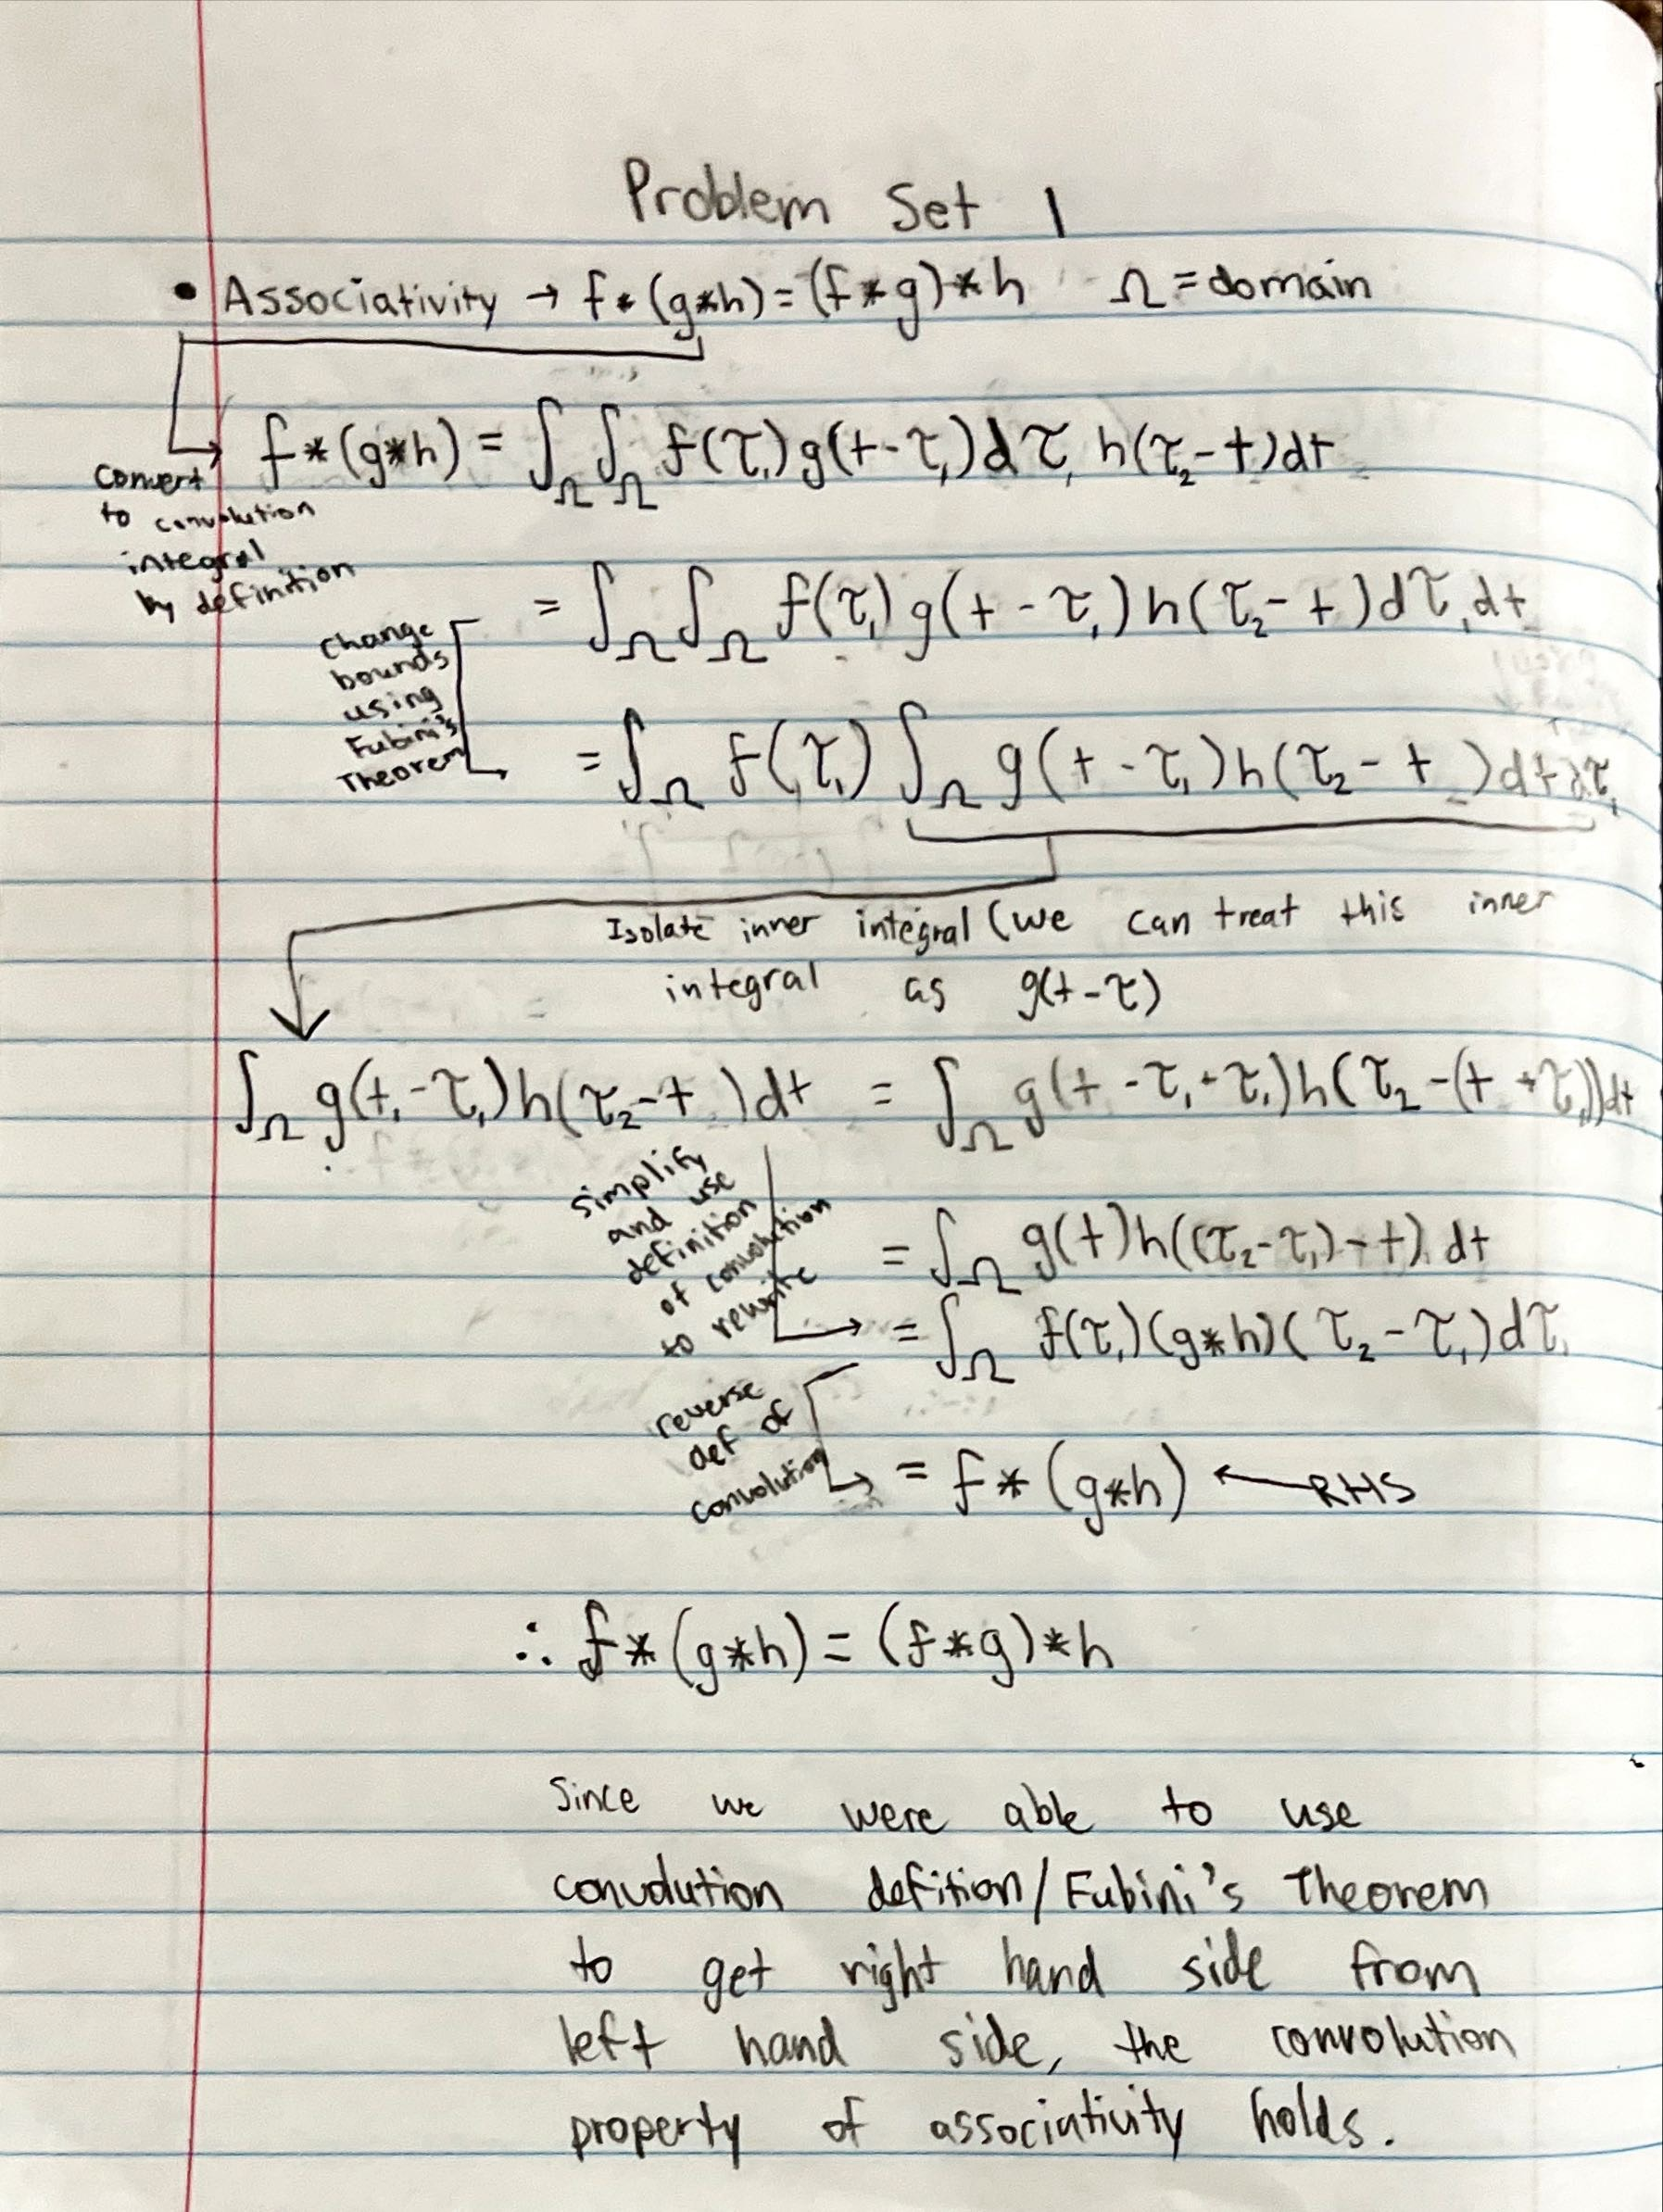
\includegraphics[scale=0.18]{Associativity.jpeg}\\\\



%\noindent We can substitute this integral such that f, g, and h are all functions of t. On the left hand side, we will plug in f and g as their respective functions in the convolution integral. On the right hand side, we will plug in g as f and h as g. \\

%\noindent We get the following:
%\begin{center}
%\textls[180]{\large{\indent$\mathcal{\int_{-\infty}^{\infty}} f(\tau)g(t-\tau)d\tau$}\\} %Definition of Convolution
%\end{center}

• Distributive: $f*(g+h) = f*g + f*h$\\\\
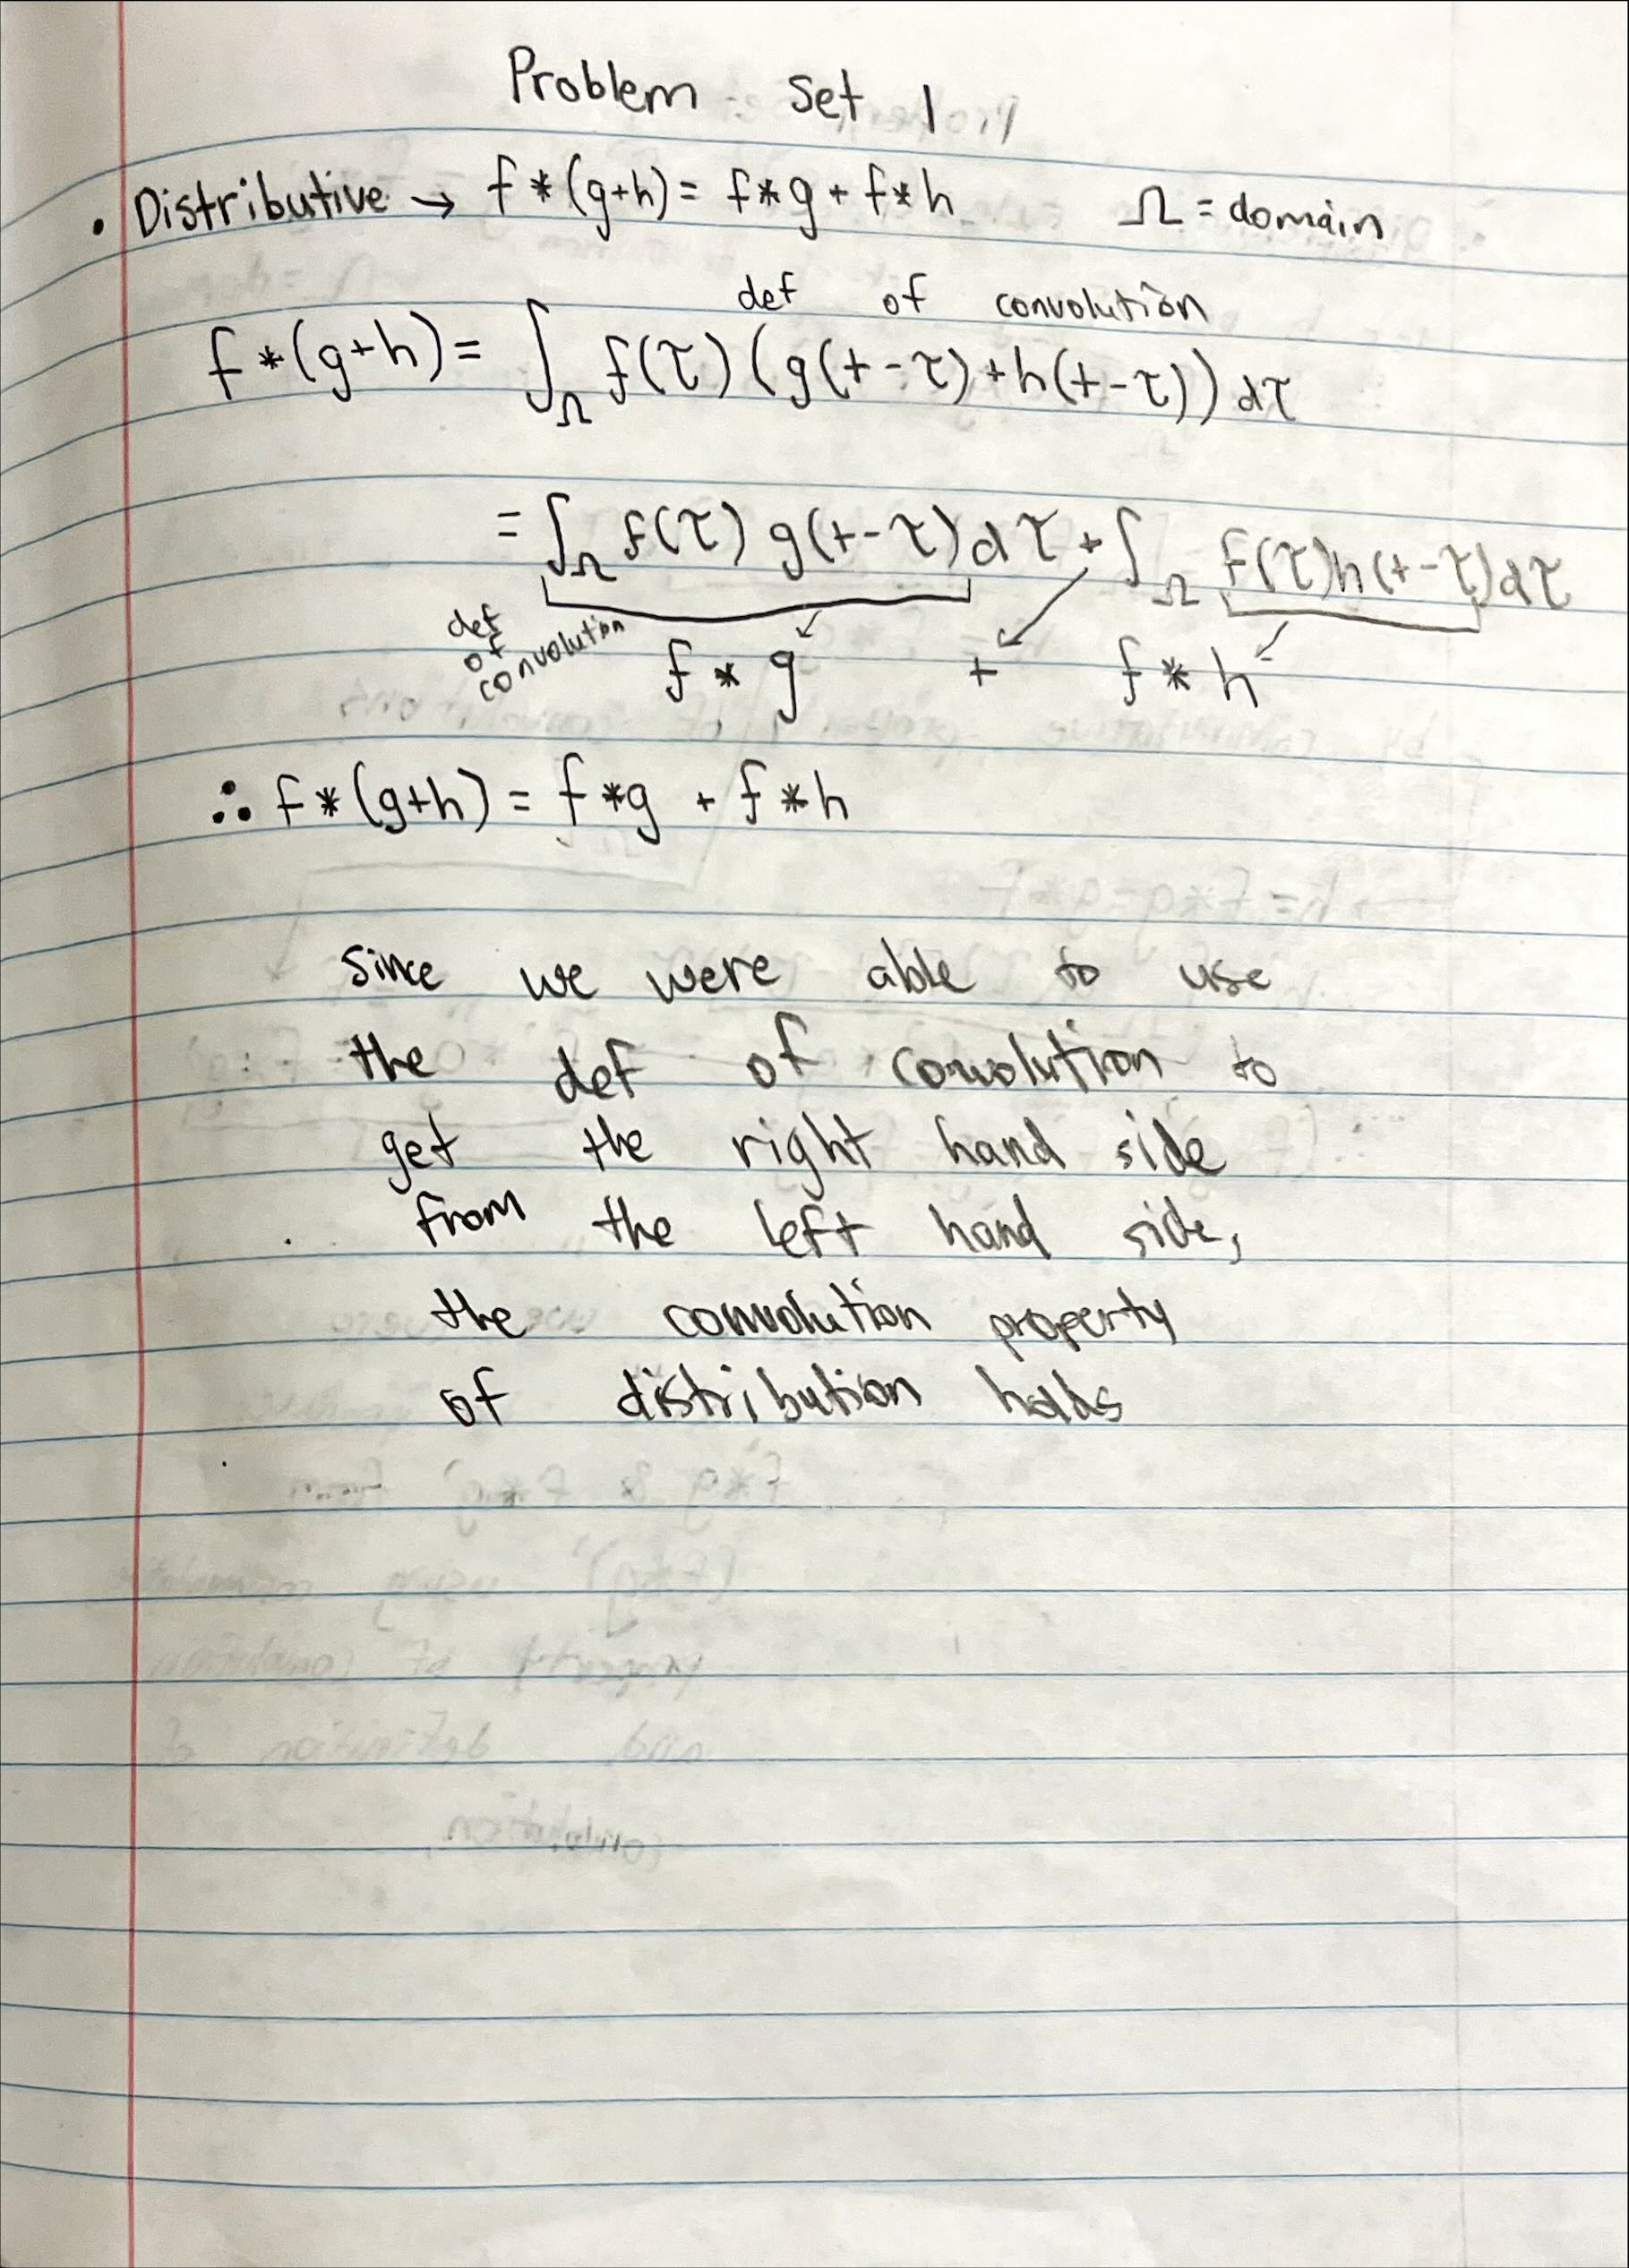
\includegraphics[scale=0.23]{Distributive.jpeg}\\\\\\
• Differentiation rule: $(f*g)' = f'*g = f * g'$\\\\
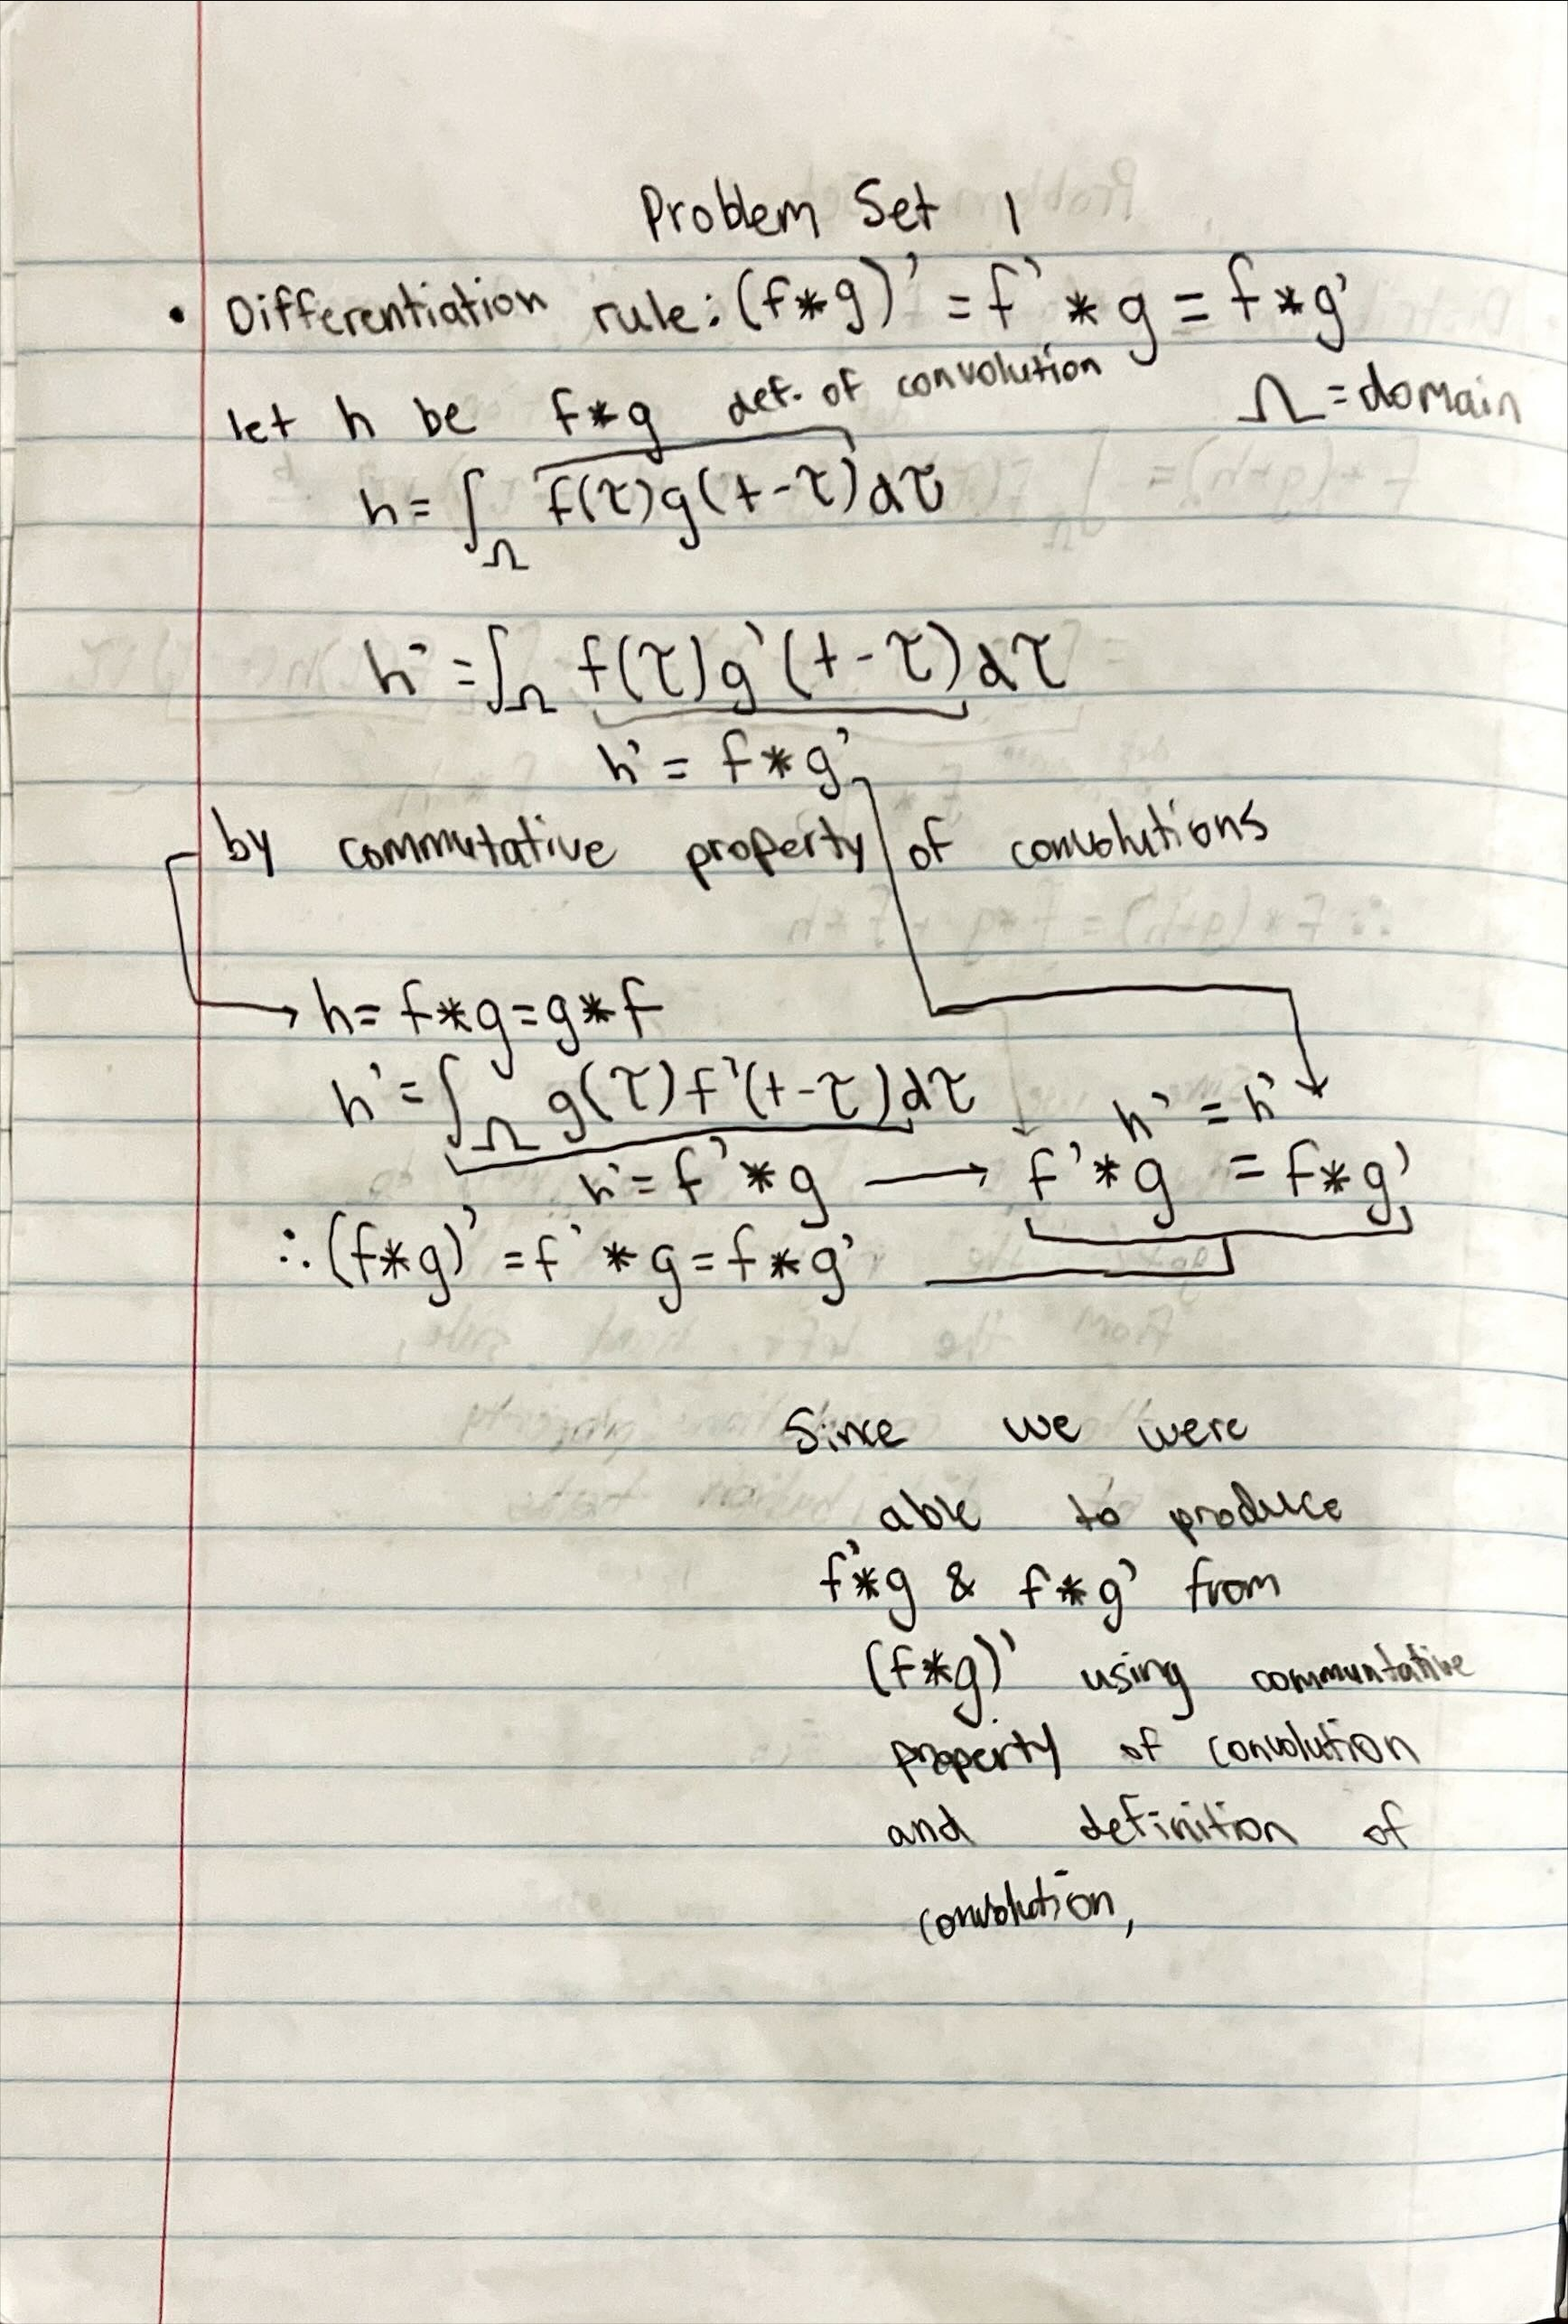
\includegraphics[scale=0.22]{Differentiation.jpeg}\\\\\\\\
• Convolution theorem: $\mathcal{F}(g*h) = \mathcal{F}(g) \mathcal{F}(h)$, where $\mathcal{F}$
 denotes Fourier transform\\\\
 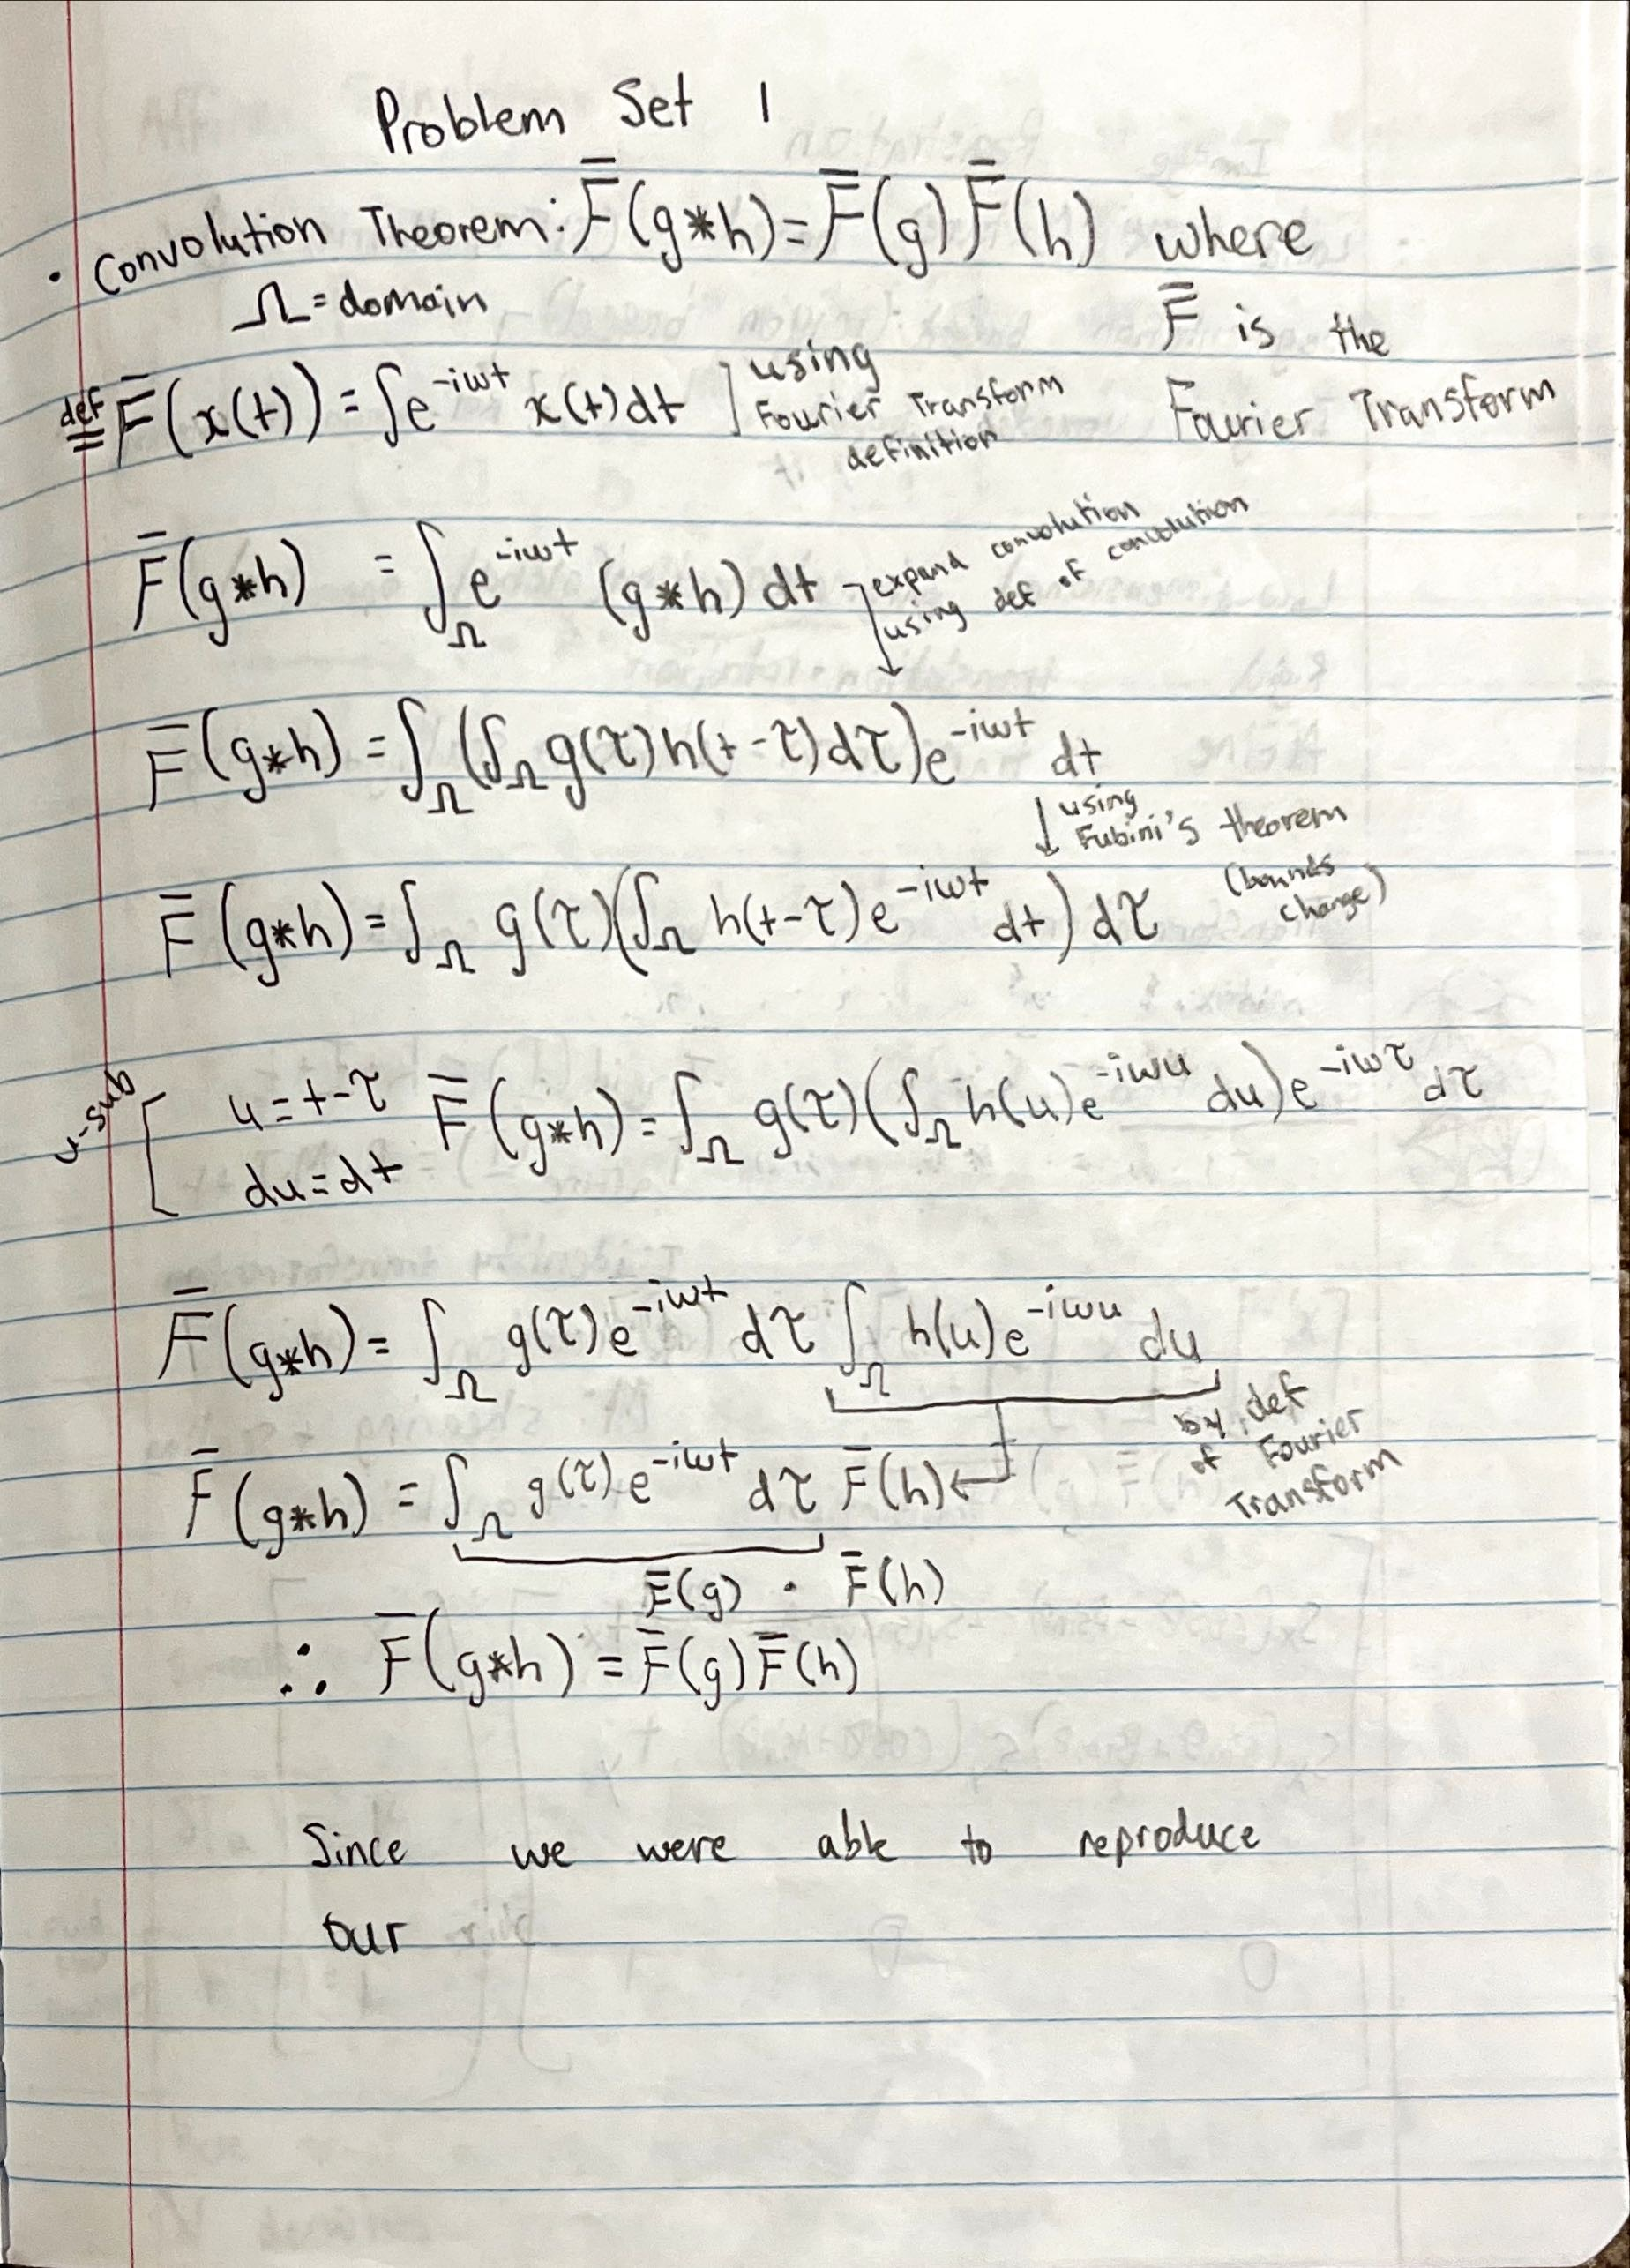
\includegraphics[scale=0.23]{Fourier.jpeg}\\

\noindent\section*{Problem 2}

\noindent \emph {a.) Compute Fourier transform of the given image lenaNoise.PNG by using fft2 function
in Matlab (or numpy.fft.fft2 in Python), and then center the low frequencies (e.g., by
using fftshift). }\\

\noindent In order to compute the Fourier Transform of a 2d image within Python, we can use numpy.fft.fft2(img) where img refers to the image we input.\\

\noindent First, lets start with our imports.
\;
\;

\begin{mdframed}[backgroundcolor=bg]
\begin{minted}{python}
import numpy as np
import matplotlib.pyplot as plt
import cv2
\end{minted}
\end{mdframed}
\;
\;

\noindent Matplotlib.pypplot will be extremely helpful in the input and output of our image. We will be able to use functions like .imread() in order to read in our image and functions like .imshow() and .show() in order to display our image.\\

\noindent Numpy and cv2 will be useful in order to perform different processing functions on our images. We will be able to use such packages to perform Fourier Transforms (to convert our image matrix into the frequency domain), as well as to create and process with masks. We will reuse these packages will be used in all parts in problem 2 and problem 3.\\

\noindent Let's now read in our input image 'lena.png'.\\

\begin{mdframed}[backgroundcolor=bg]
\begin{minted}{python}
lenaImage = plt.imread('lena.png')
\end{minted}
\end{mdframed}
\;
\;


\noindent Next, we'll compute the Fourier transform with np.fft.fft2. We will also use fftshift to center the low frequencies in the image.\\

\begin{mdframed}[backgroundcolor=bg]
\begin{minted}{python}
#Perform's fourier transform on lena image
ftShift = np.fft.fftshift(np.fft.fft2(lenaImage, axes=(0,1)))
ftShift2 = np.fft.fftshift(np.fft.fft2(lenaImage, axes=(0,1)))
ftShift3 = np.fft.fftshift(np.fft.fft2(lenaImage, axes=(0,1))) 
\end{minted}
\end{mdframed}
\;
\;
\pagebreak\\\\

\noindent Finally, we use subplots to find our output.
\begin{mdframed}[backgroundcolor=bg]
\begin{minted}{python}
fig, ax = plt.subplots(1,2)
fig.suptitle('PART A')
fig. set_size_inches((12, 8)) #Increases window size

#Setup Figure/Subplots
ax[0].imshow(lenaImage)
ax[0].set_title("Original Image", fontsize=5)
ax[1].imshow(np.log(np.abs(ftShift)))
ax[1].set_title("Fourier Transform (Centered low frequencies)",fontsize=5)
plt.show()
\end{minted}
\end{mdframed}
\;
\;

\noindent We get the following output from our code so far for part A:\\\\
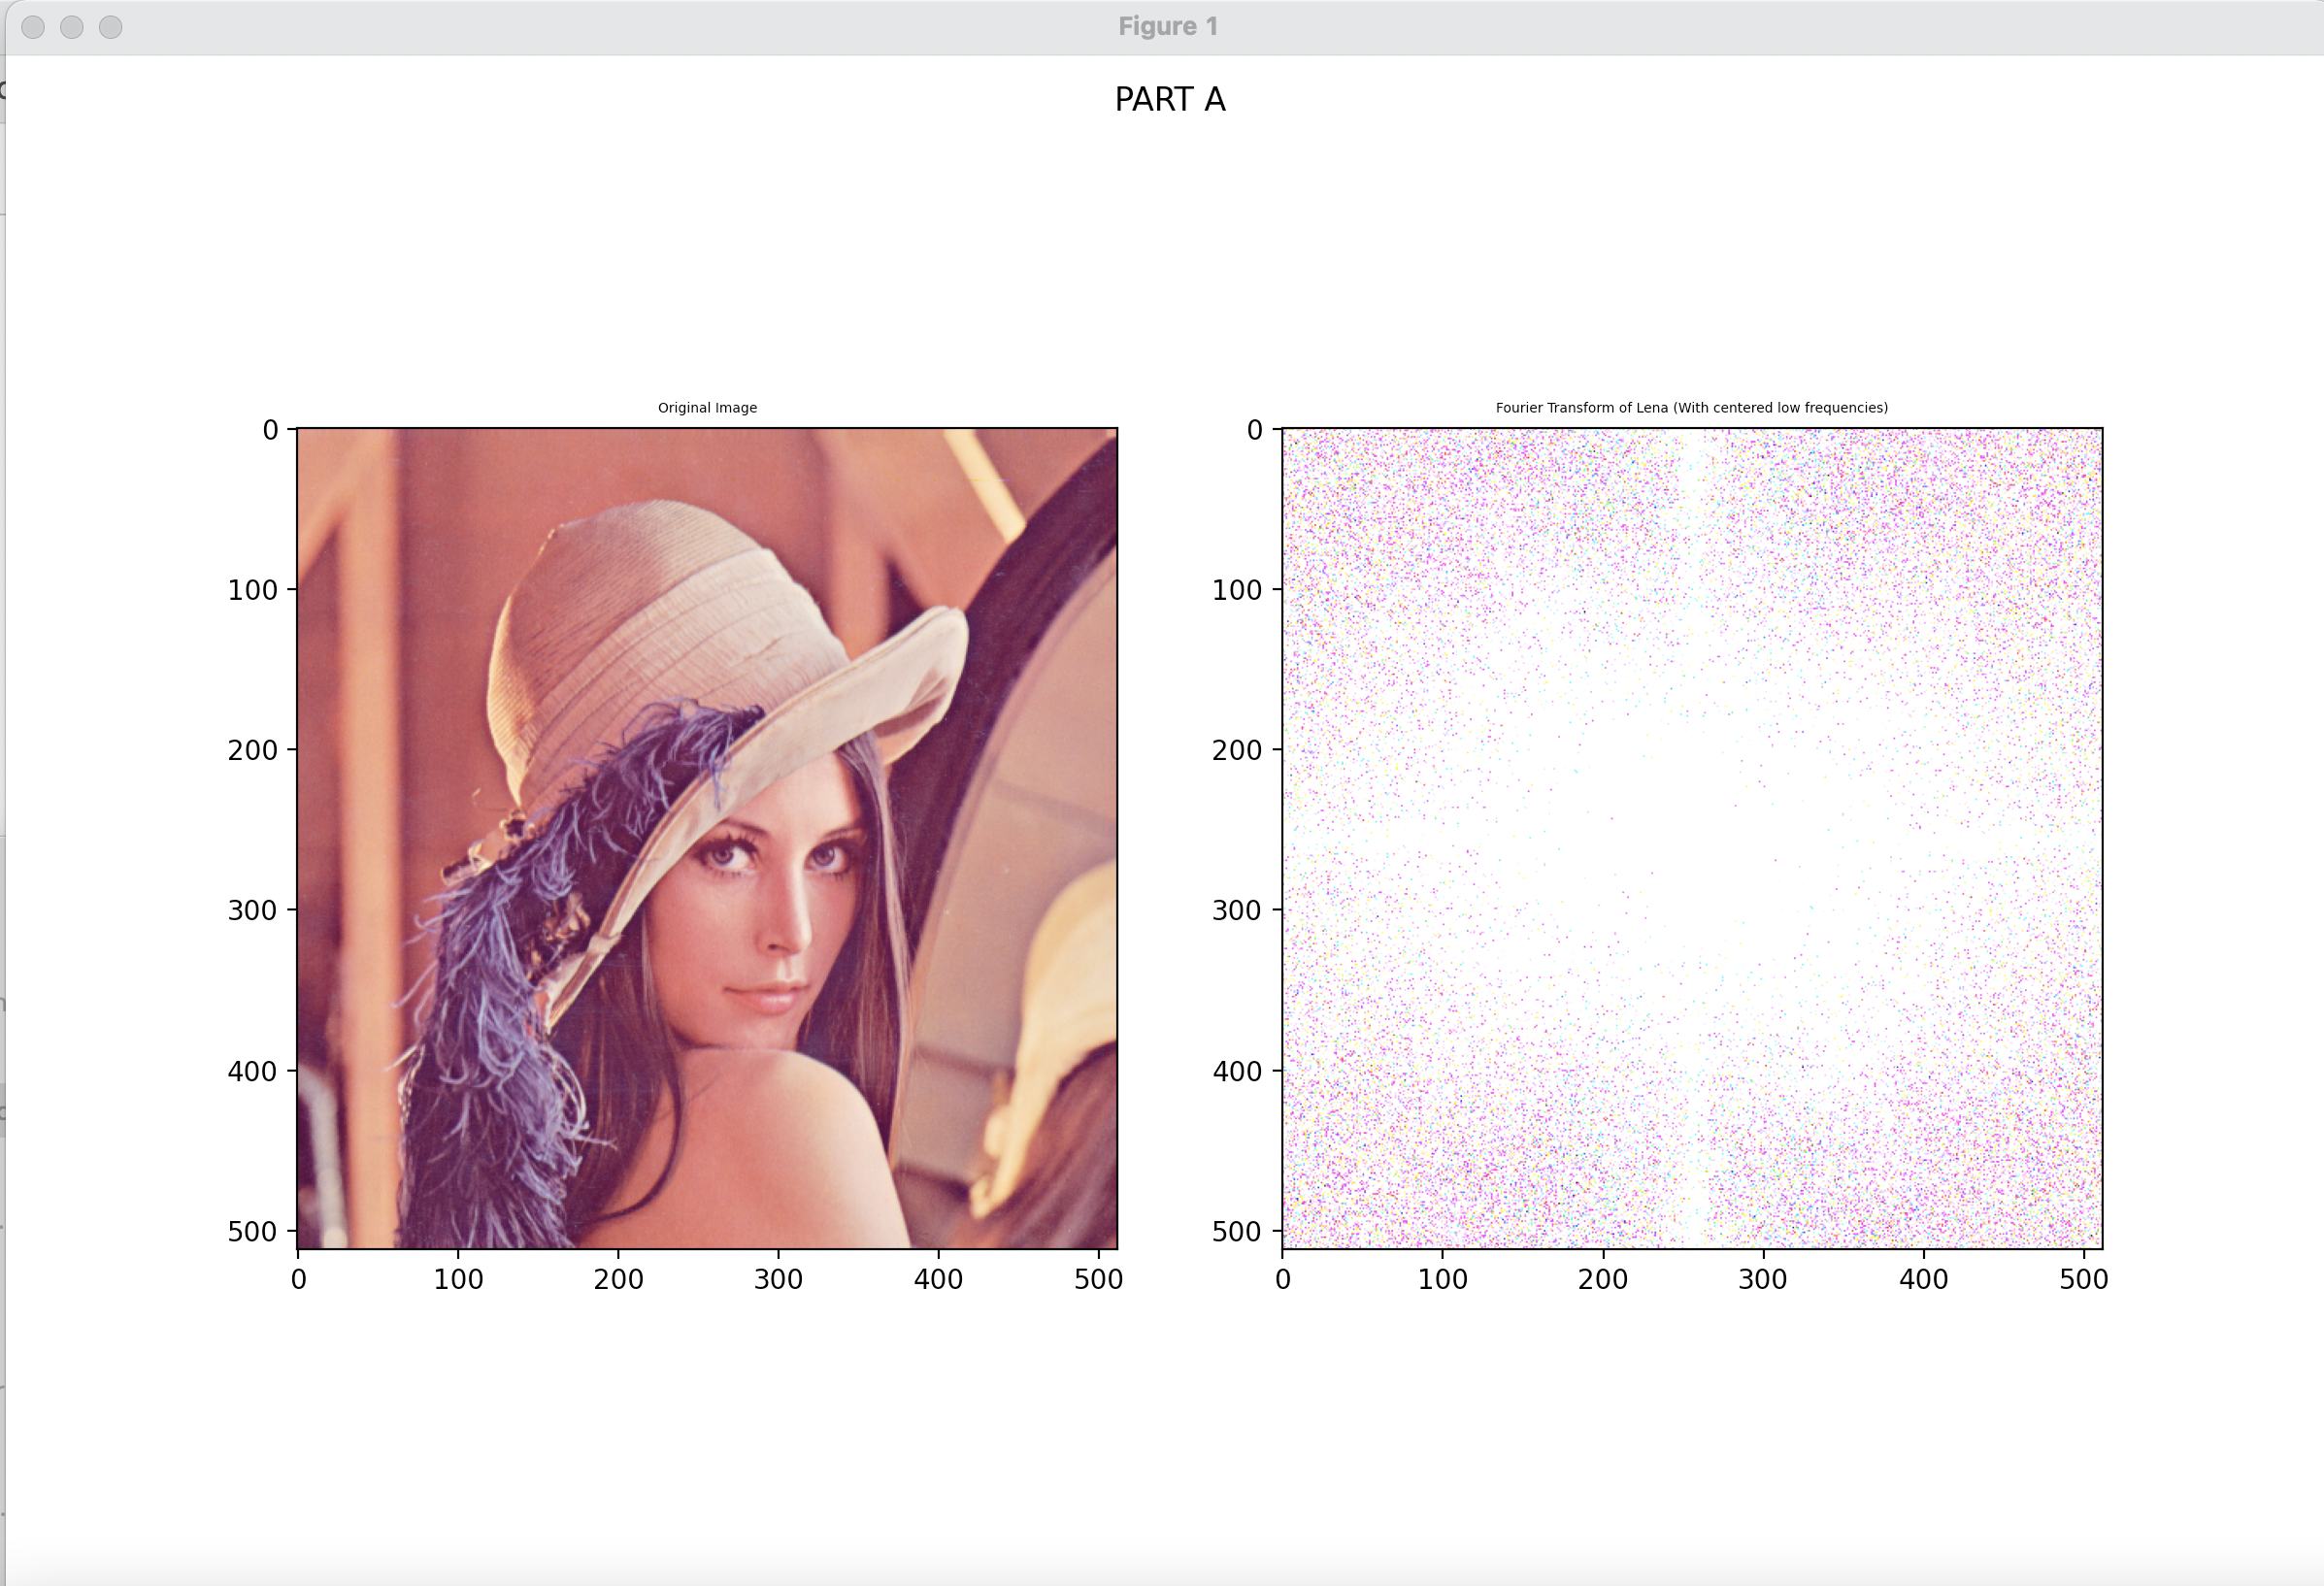
\includegraphics[scale=0.4]{2A.png}\\\\
\pagebreak\\\\\\
\noindent \emph { (b) Keep different number of low frequencies (e.g., $10^2$; $20^2$; $40^2$ and the full dimension), but set all other high frequencies to 0.
(c) Reconstruct the original image (ifft2) by using the new generated frequencies in step
(b).}\\\\
\;
\;
\noindent For simplicity's sake, we will combine part B and part C into the following explanation. We include code review for both parts as well as the output for each below.\\

\noindent For part B, we can create rectangular masks using cv2.rectangle and apply them to our Fourier transforms from part A. Certain parts are shortened intentionally (especially comments) in order to fit the constraints of the code block. \\

\begin{mdframed}[backgroundcolor=bg]
\begin{minted}{python}
mask40 = np.zeros_like(lenaImage)
mask20 = np.zeros_like(lenaImage)
mask10 = np.zeros_like(lenaImage)

x = int(mask40.shape[1]/2) #CenterX of frquency domain
y = int(mask40.shape[0]/2) #CenterY of frquency domain

#Mask Fourier transforms with rect to 0 out high frequencies 
cv2.rectangle(mask40,((x-40),(y-40)),((x+40),(y+40)),(255,255,255),-1)[0]#
cv2.rectangle(mask20,((x-20),(y-20)),((x+20),(y+20)),(255,255,255),-1)[0]#
cv2.rectangle(mask10,((x-10),(y-10)),((x+10),(y+10)),(255,255,255),-1)[0]#

ftShift *= mask40/255
ftShift2 *= mask20/255
ftShift3 *= mask10/255
\end{minted}
\end{mdframed}\\\\
\;

\noindent We use the following three rectangles to mask the frequency domain of our lena image, eliminating certain frequencies from our image. Mask40 masks with a square of side length 40, mask20 masks with a square of side length 20, and mask10 masks with a square of side length 10. We preserve the middle, low frequencies by setting our inside of our square to white, while eliminating our high frequencies outside the square by leaving it black.\\

\noindent For part C, we use np.fft.ifftshift to inverse our fftshift and np.fft.ifft2 to convert back from the frequency domain to our spatial domain. We finally use the absolute value in order to regularize our domain to try to get our true, previous values back especially for intensity.

\pagebreak\\\\
\begin{mdframed}[backgroundcolor=bg]
\begin{minted}{python}
#Reconstruct original image using inverse fourier transform
reconstructed=np.abs(np.fft.ifft2(np.fft.ifftshift(ftShift),axes=(0,1))) 
reconstructed2=np.abs(np.fft.ifft2(np.fft.ifftshift(ftShift2),axes=(0,1))) 
reconstructed3=np.abs(np.fft.ifft2(np.fft.ifftshift(ftShift3),axes=(0,1))) 
#Setup Figure/Subplots
fig, ax = plt.subplots(1,4)
fig.suptitle('PART B & C')
fig.set_size_inches((12, 8)) #Increases window size

ax[0].imshow(lenaImage)
ax[0].set_title("Original Image", fontsize=5)
ax[1].imshow(reconstructed)
ax[1].set_title("Lena image removing frequencies beyond 40^2", fontsize=5)
ax[2].imshow(reconstructed2)
ax[2].set_title("Lena image removing frequencies beyond 20^2", fontsize=5)
ax[3].imshow(reconstructed3)
ax[3].set_title("Lena image removing frequencies beyond 10^2", fontsize=5)
plt.show()
\end{minted}
\end{mdframed}
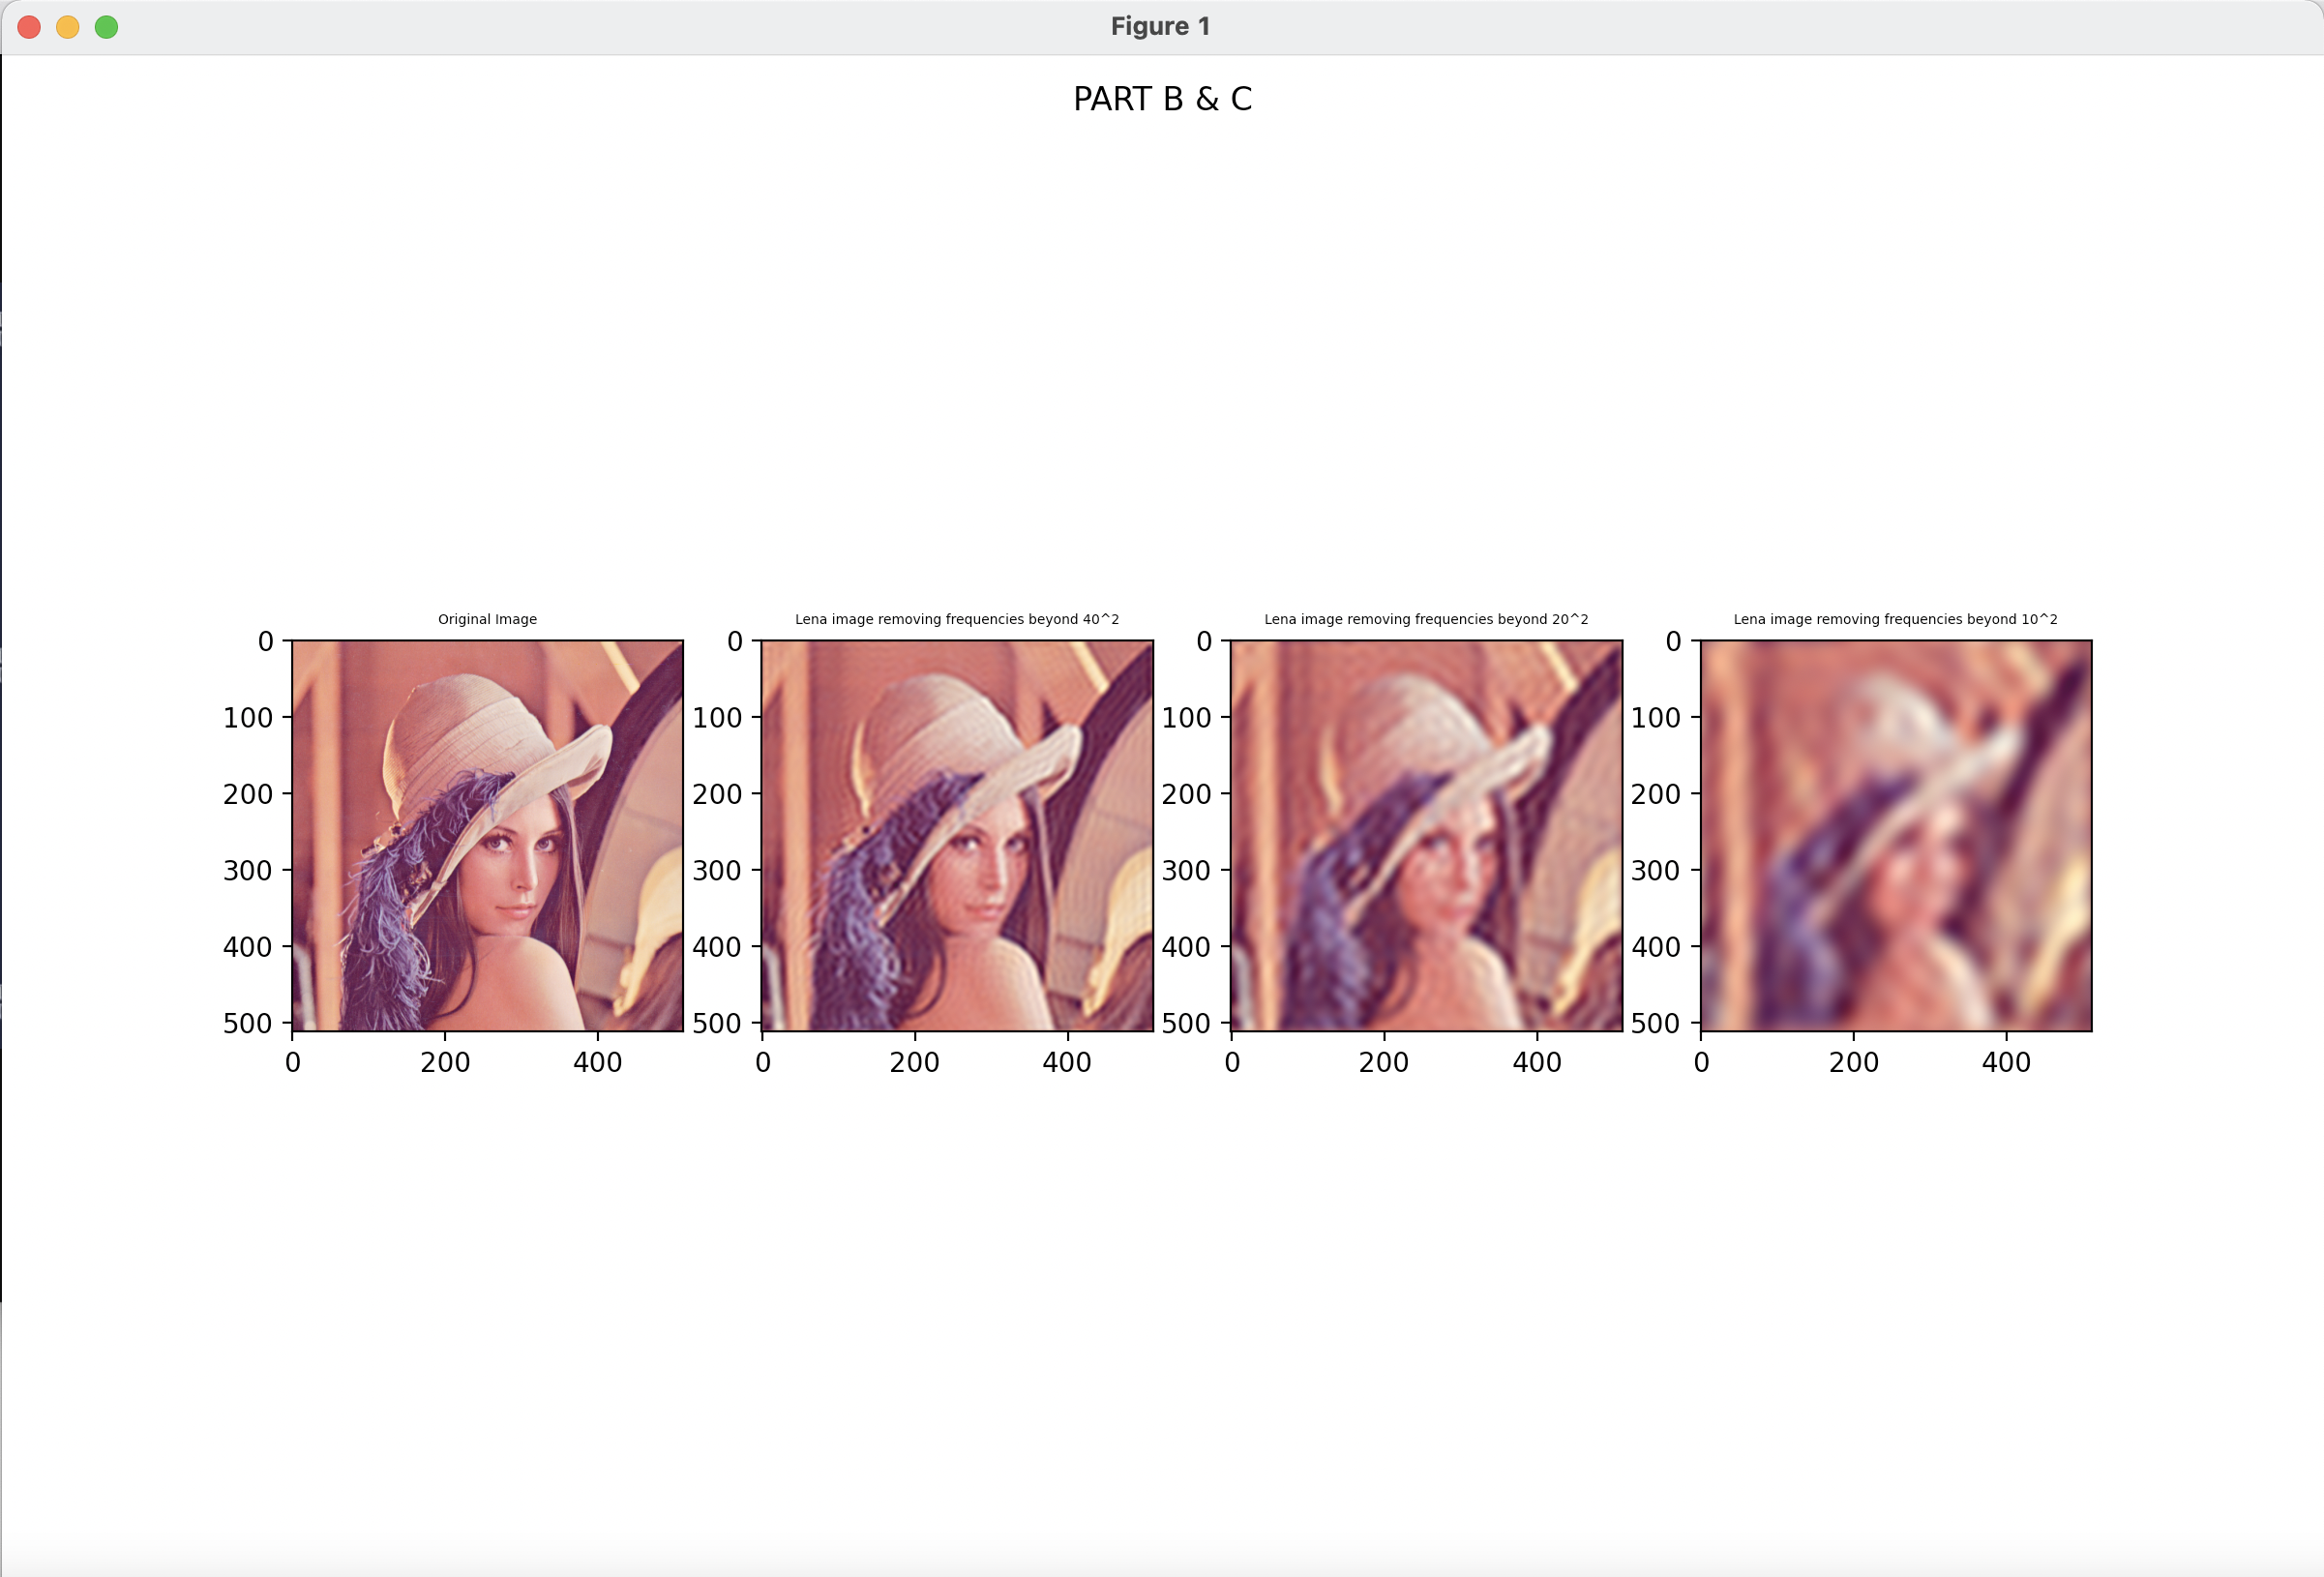
\includegraphics[scale=0.38]{2B&C.png}\\

\noindent From left to right, we plot the original image, and then the images with frequencies beyond $40^2$,$20^2$,and $10^2$ removed respectively.
\pagebreak\\

\noindent\section*{Problem 3}

\noindent Finally, we move on to implmenting gradient descent. We are tasked with implementing a gradient descent algorithm for a ROF model with total variation minimization, capable of denoising a 2D image.\\

\noindent First, lets showcase our given functions. Forward difference x and y determines the changes in x and y, which computes a component for the gradient of u.\\

\begin{mdframed}[backgroundcolor=bg]
\begin{minted}{python}
 def gaussian_noise(self,img_gray,sigma): #Applies noise to an image
    row,col= img_gray.shape
    mean = 0
    var = sigma
    sigma = var ** 0.3
    gaussian = np.random.normal(mean, sigma, (row, col)) 
    noisy_img = img_gray + gaussian
    return noisy_img

def forward_difference_x(self,image): #Computes the x comp of gradient
    rows, cols = image.shape
    d = np.zeros((rows,cols))
    d[:,1:cols-1] = image[:,1:cols-1] - image[:,0:cols-2]
    d[:,0] = image[:,0] - image[:,cols-1]
    return d

def forward_difference_y(self,image): #Computes the y comp of gradient
    rows, cols = image.shape
    d = np.zeros((rows,cols))
    d[1:rows-1, :] = image[1:rows-1, :] - image[0:rows-2, :]
    d[0,:] = image[0,:] - image[rows-1,:]
    return d
\end{minted}
\end{mdframed}

\noindent For our gradient descent algorithm, we create the following methods below. Our magnitude function takes the magnitude of a matrix with a L2 norm (a 2D matrix). Our gradient function computes the gradient of our energy function. Dx/Dy are used to shorten the names of forward difference x/y, and du is used in the denominator of when we compute the gradient/divergence of our u, such that our u is our image undergoing denoising. Last but not least, our div function computes the gradient/divergence operator of our u.

\pagebreak\\
\begin{mdframed}[backgroundcolor=bg]
\begin{minted}{python}
def magnitude(self,matrix): #Determines the magnitude of a 2D matrix
    return np.linalg.norm(matrix,ord=2)

def gradient(self, u, img, LAMBDA, EPSILON): #Energy gradient 
    return (-2 * LAMBDA *(img - u)-self.div(img, EPSILON))

def dx(self, x): #Determines fowardX, shortens name
    return self.forward_difference_x(x) 

def dy(self, y): #Determines fowardY differences, shortens name
    return self.forward_difference_y(y)

def du(self, u,epsilon): #Denominator used in divergence function (div)
     return np.sqrt(self.dx(u)**2 + self.dy(u)**2)+epsilon 

def div(self, u, epsilon): #Detemines the divergence of u 
    return self.dx(np.divide(self.dx(u),self.du(u,epsilon)))+
           self.dy((np.divide(self.dy(u),self.du(u, epsilon)))
\end{minted}
\end{mdframed}
\;
\;

\noindent Next, we show our definitions of our hyperparameters. These regulate and determine the speed and effectiveness in which we perform gradient descent on our image.\\

\begin{mdframed}[backgroundcolor=bg]
\begin{minted}{python}
ITERATIONS = 100 #Max iterations
LAMBDA = 0.9 #Scalar
ALPHA = 0.6 #Step-size/Learning Rate
EPSILON = 0.00001 #Small shift value when computing divergence
THRESHOLD = 0.1**16 #CONVERGENCE INTERVAL 
SIGMA = sigma #Noise Threshold
u0 = 0.2 #INITIAL U START
\end{minted}
\end{mdframed}
\;
\;


\noindent We now show our gradient descent algorithm. The following is a basic implementation of the gradient descent algorithm. We denoise our image by subtracting it by the gradient times the learning rate $\lambda$. We then check the magnitude of our gradient against the magnitude of our previous gradient to see whether our energy function is within the convergence threshold for an early break. At worst case, we run 100 iterations. \\
\pagebreak\\\\
\begin{mdframed}[backgroundcolor=bg]
\begin{minted}{python}
for k in range(1,ITERATIONS):
    #print(k)
    gradient = self.gradient(u, noised, LAMBDA, EPSILON)
    u = u - ALPHA * gradient
    
    if ( k > 5 and 
    abs(self.magnitude(gradient)-self.magnitude(prevGradient))<THRESHOLD):
        break

    convPlotX = np.append(convPlotX, k)
    convPlotY = np.append(convPlotY, self.magnitude(gradient))
    
    prevGradient = gradient.copy()

\end{minted}
\end{mdframed}
\;
\;

\noindent After testing alpha 0.1-0.7 in 0.1 increments, the gradient descent algorithm is optimized at alpha = 0.6 (least iterations). We also optimize our gradient descent algorithm by declaring convergence of our E(u) as $E(u) = 1.0*10^{-18}  \approx  0$. Using a large $ \lambda < 0.1$ is also quite helpful, and I found after testing many $\lambda$'s $0.1-0.5/0.8-0.9$ in $0.1$ increments, for $0.9$ to require the least amount of iterations to denoise.\\

\noindent The following are our results from $\sigma = 0.01$\\
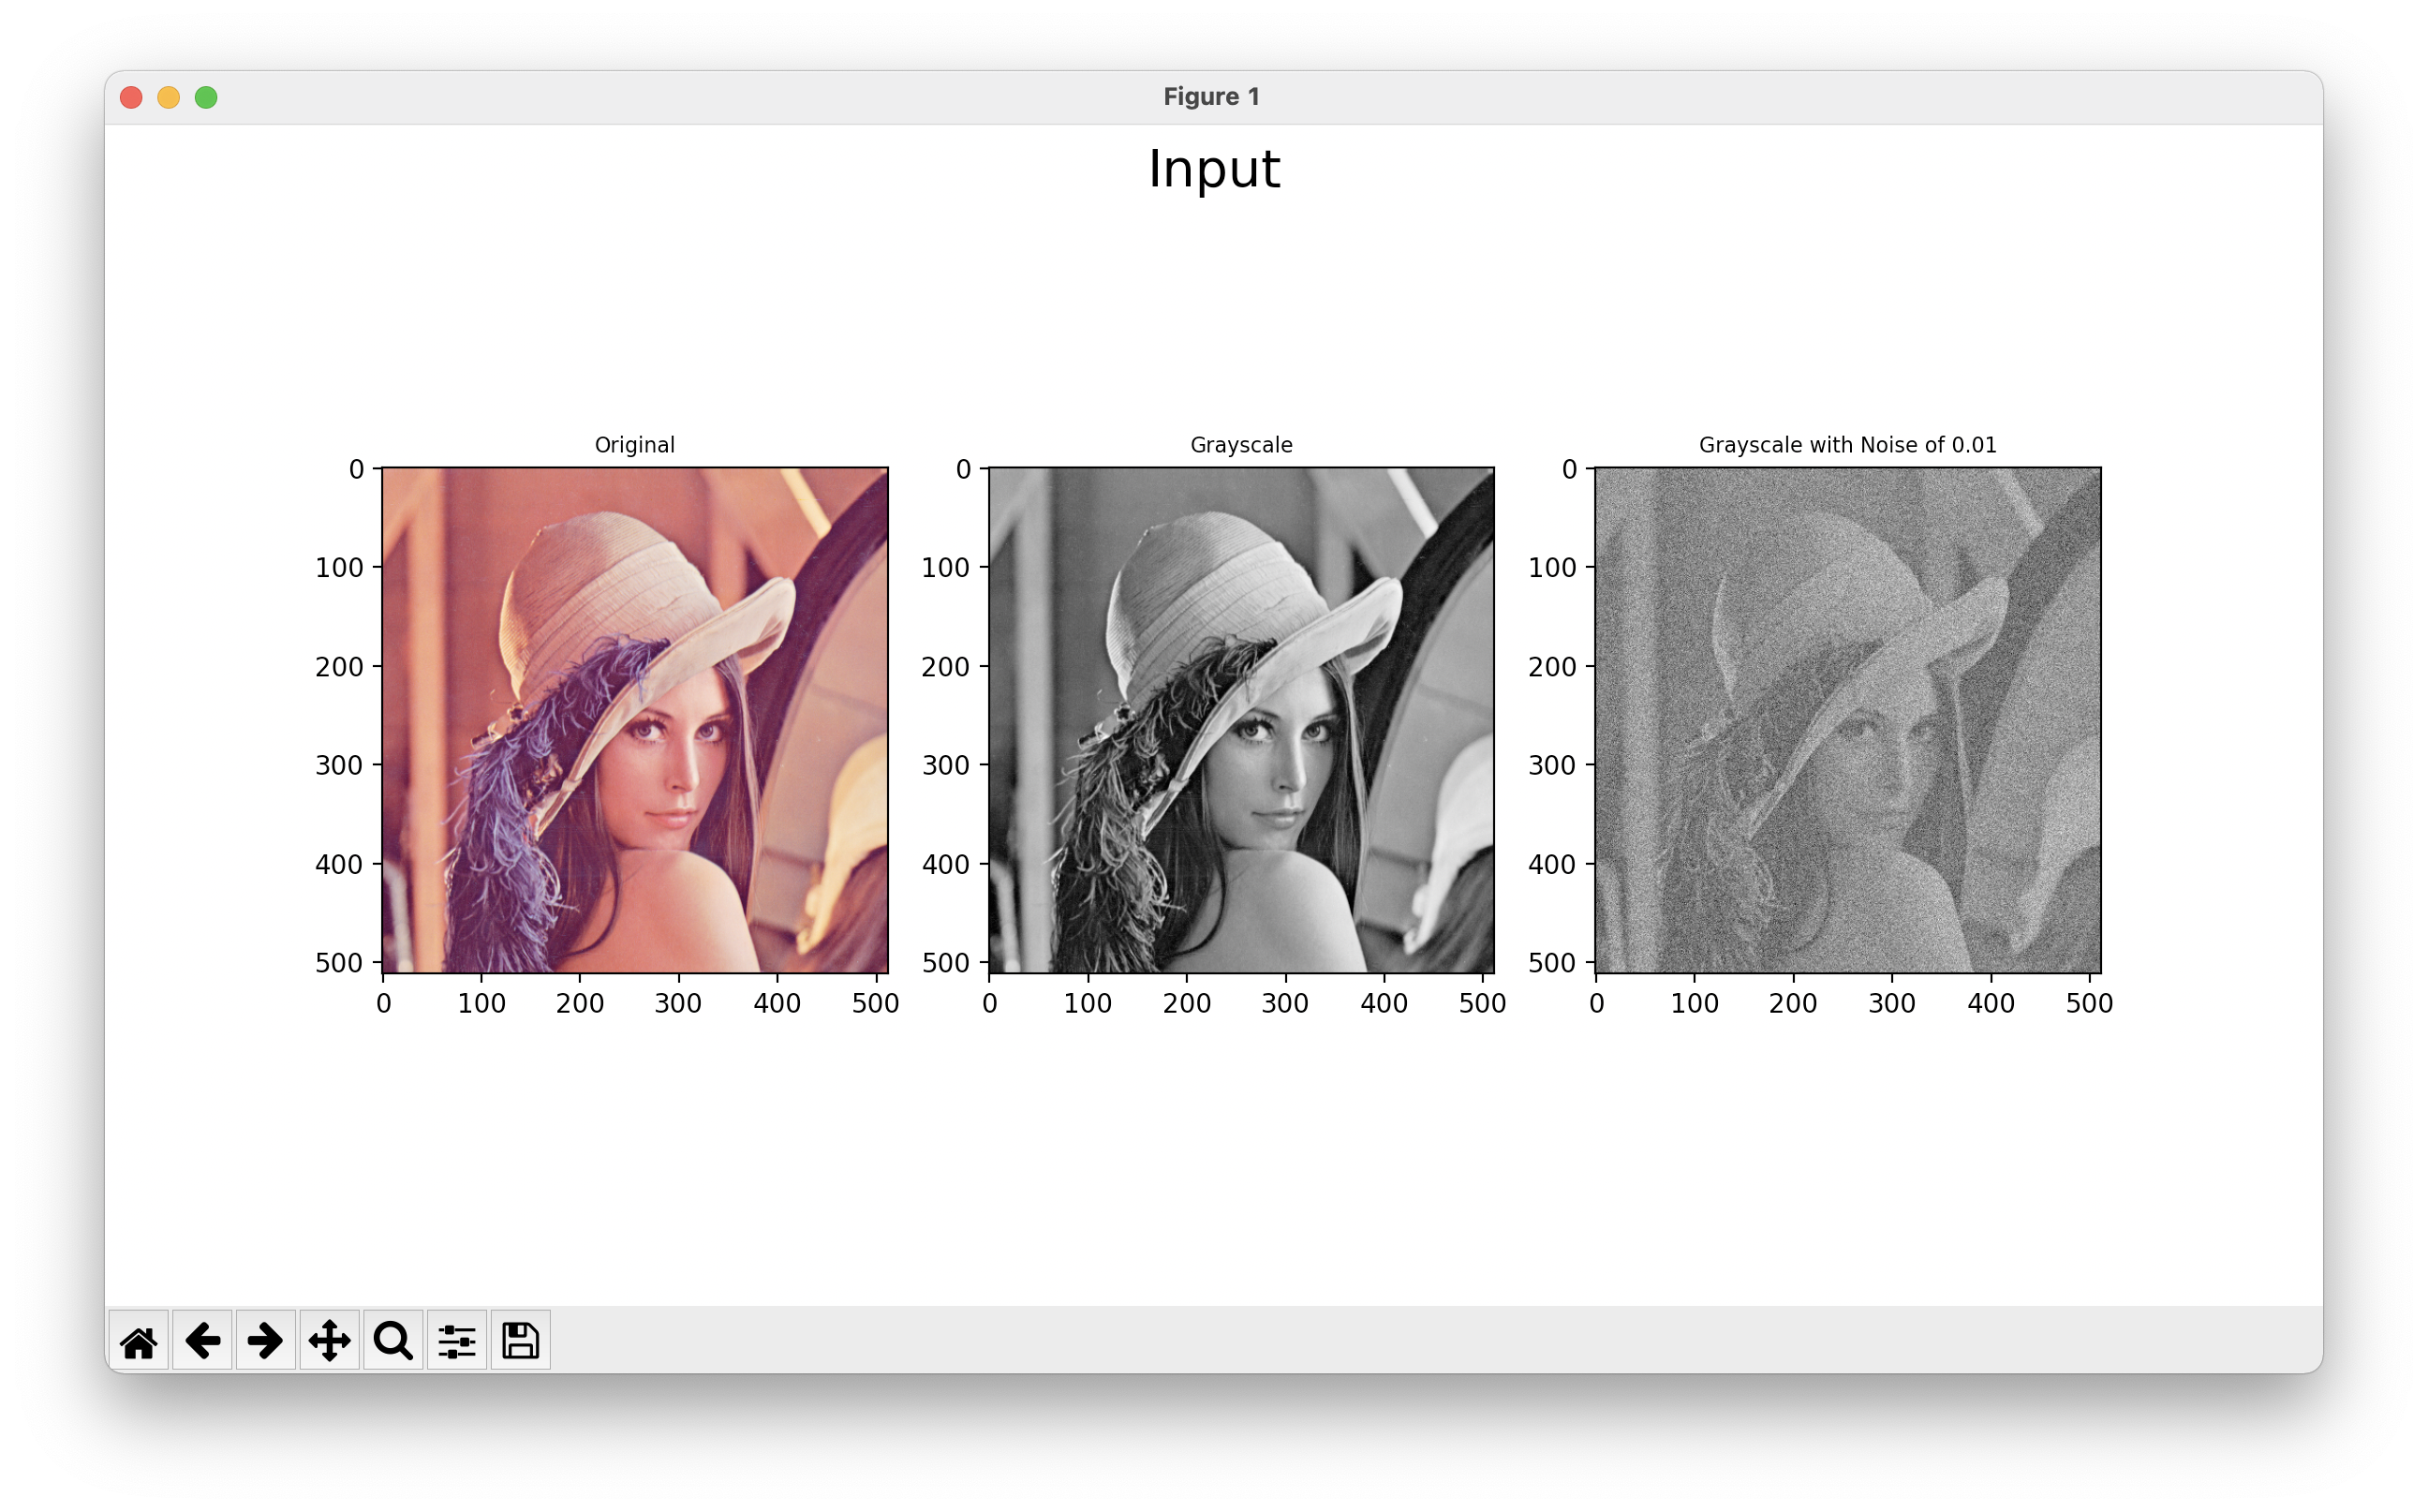
\includegraphics[scale=0.19]{3 0.01 Noise In.png}
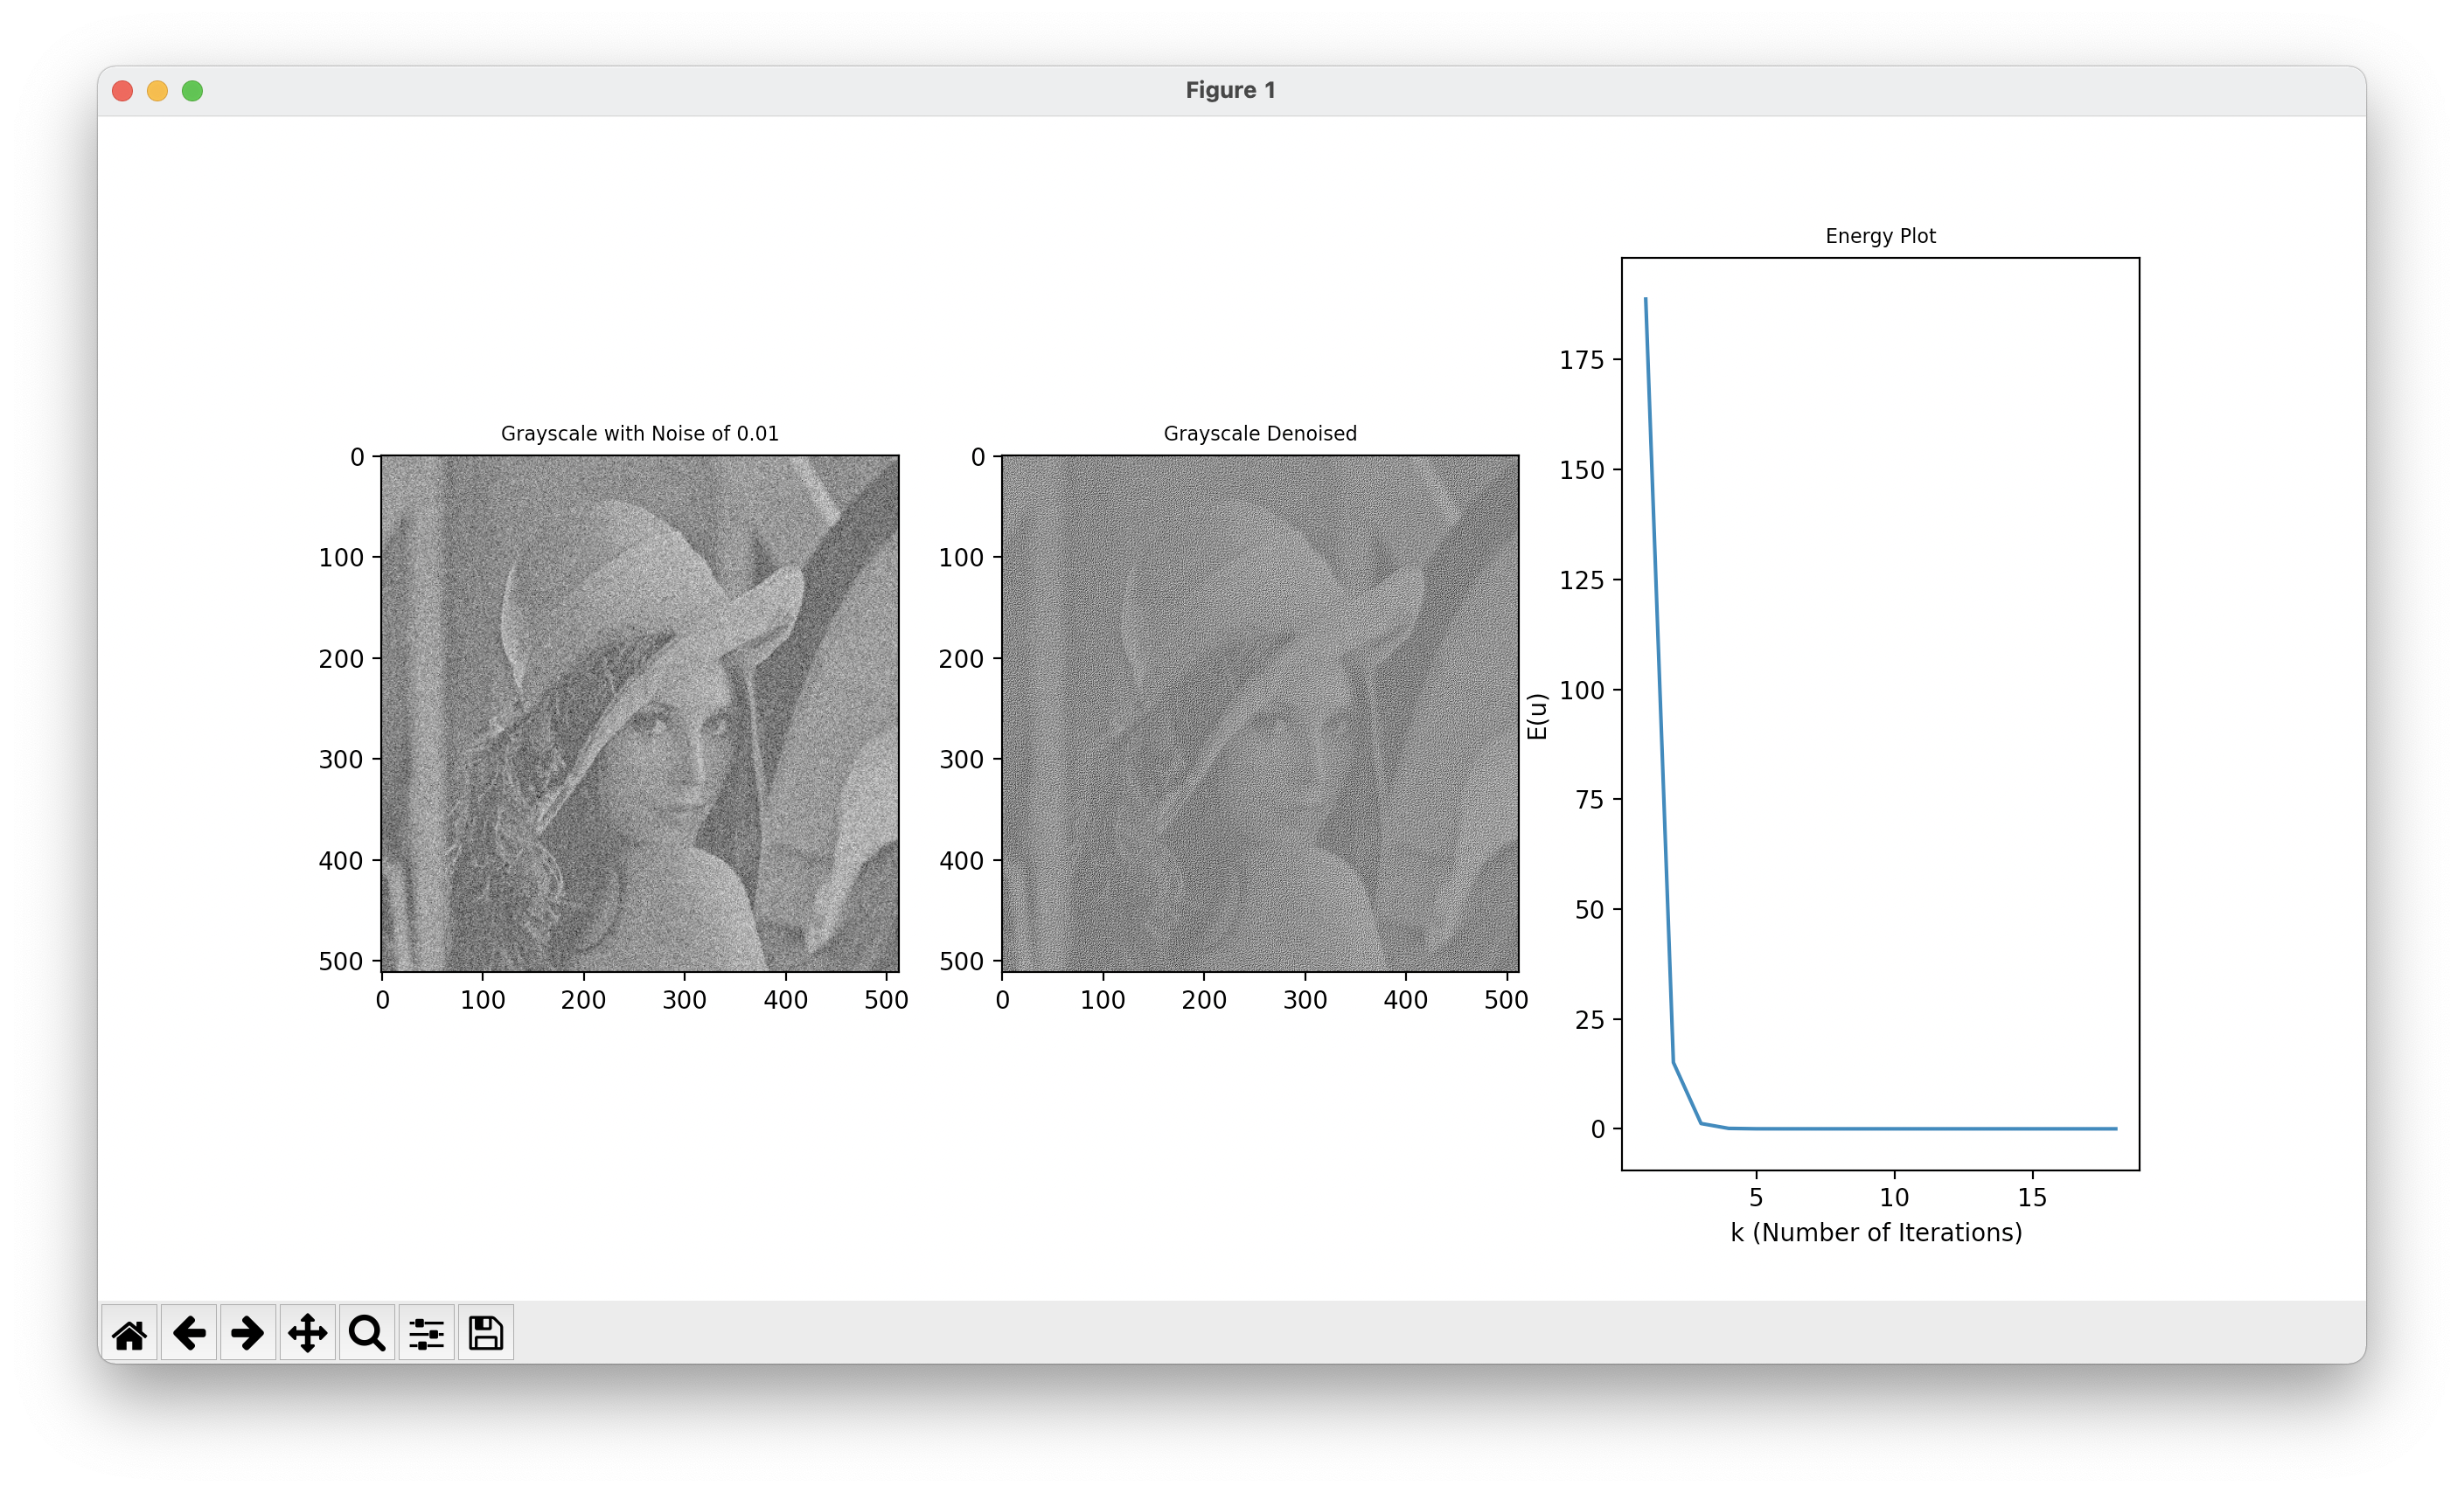
\includegraphics[scale=0.18]{3 0.01 Noise Out.png}\\\\
\pagebreak\\\\\\
\noindent The following are our results from $\sigma = 0.05$\\
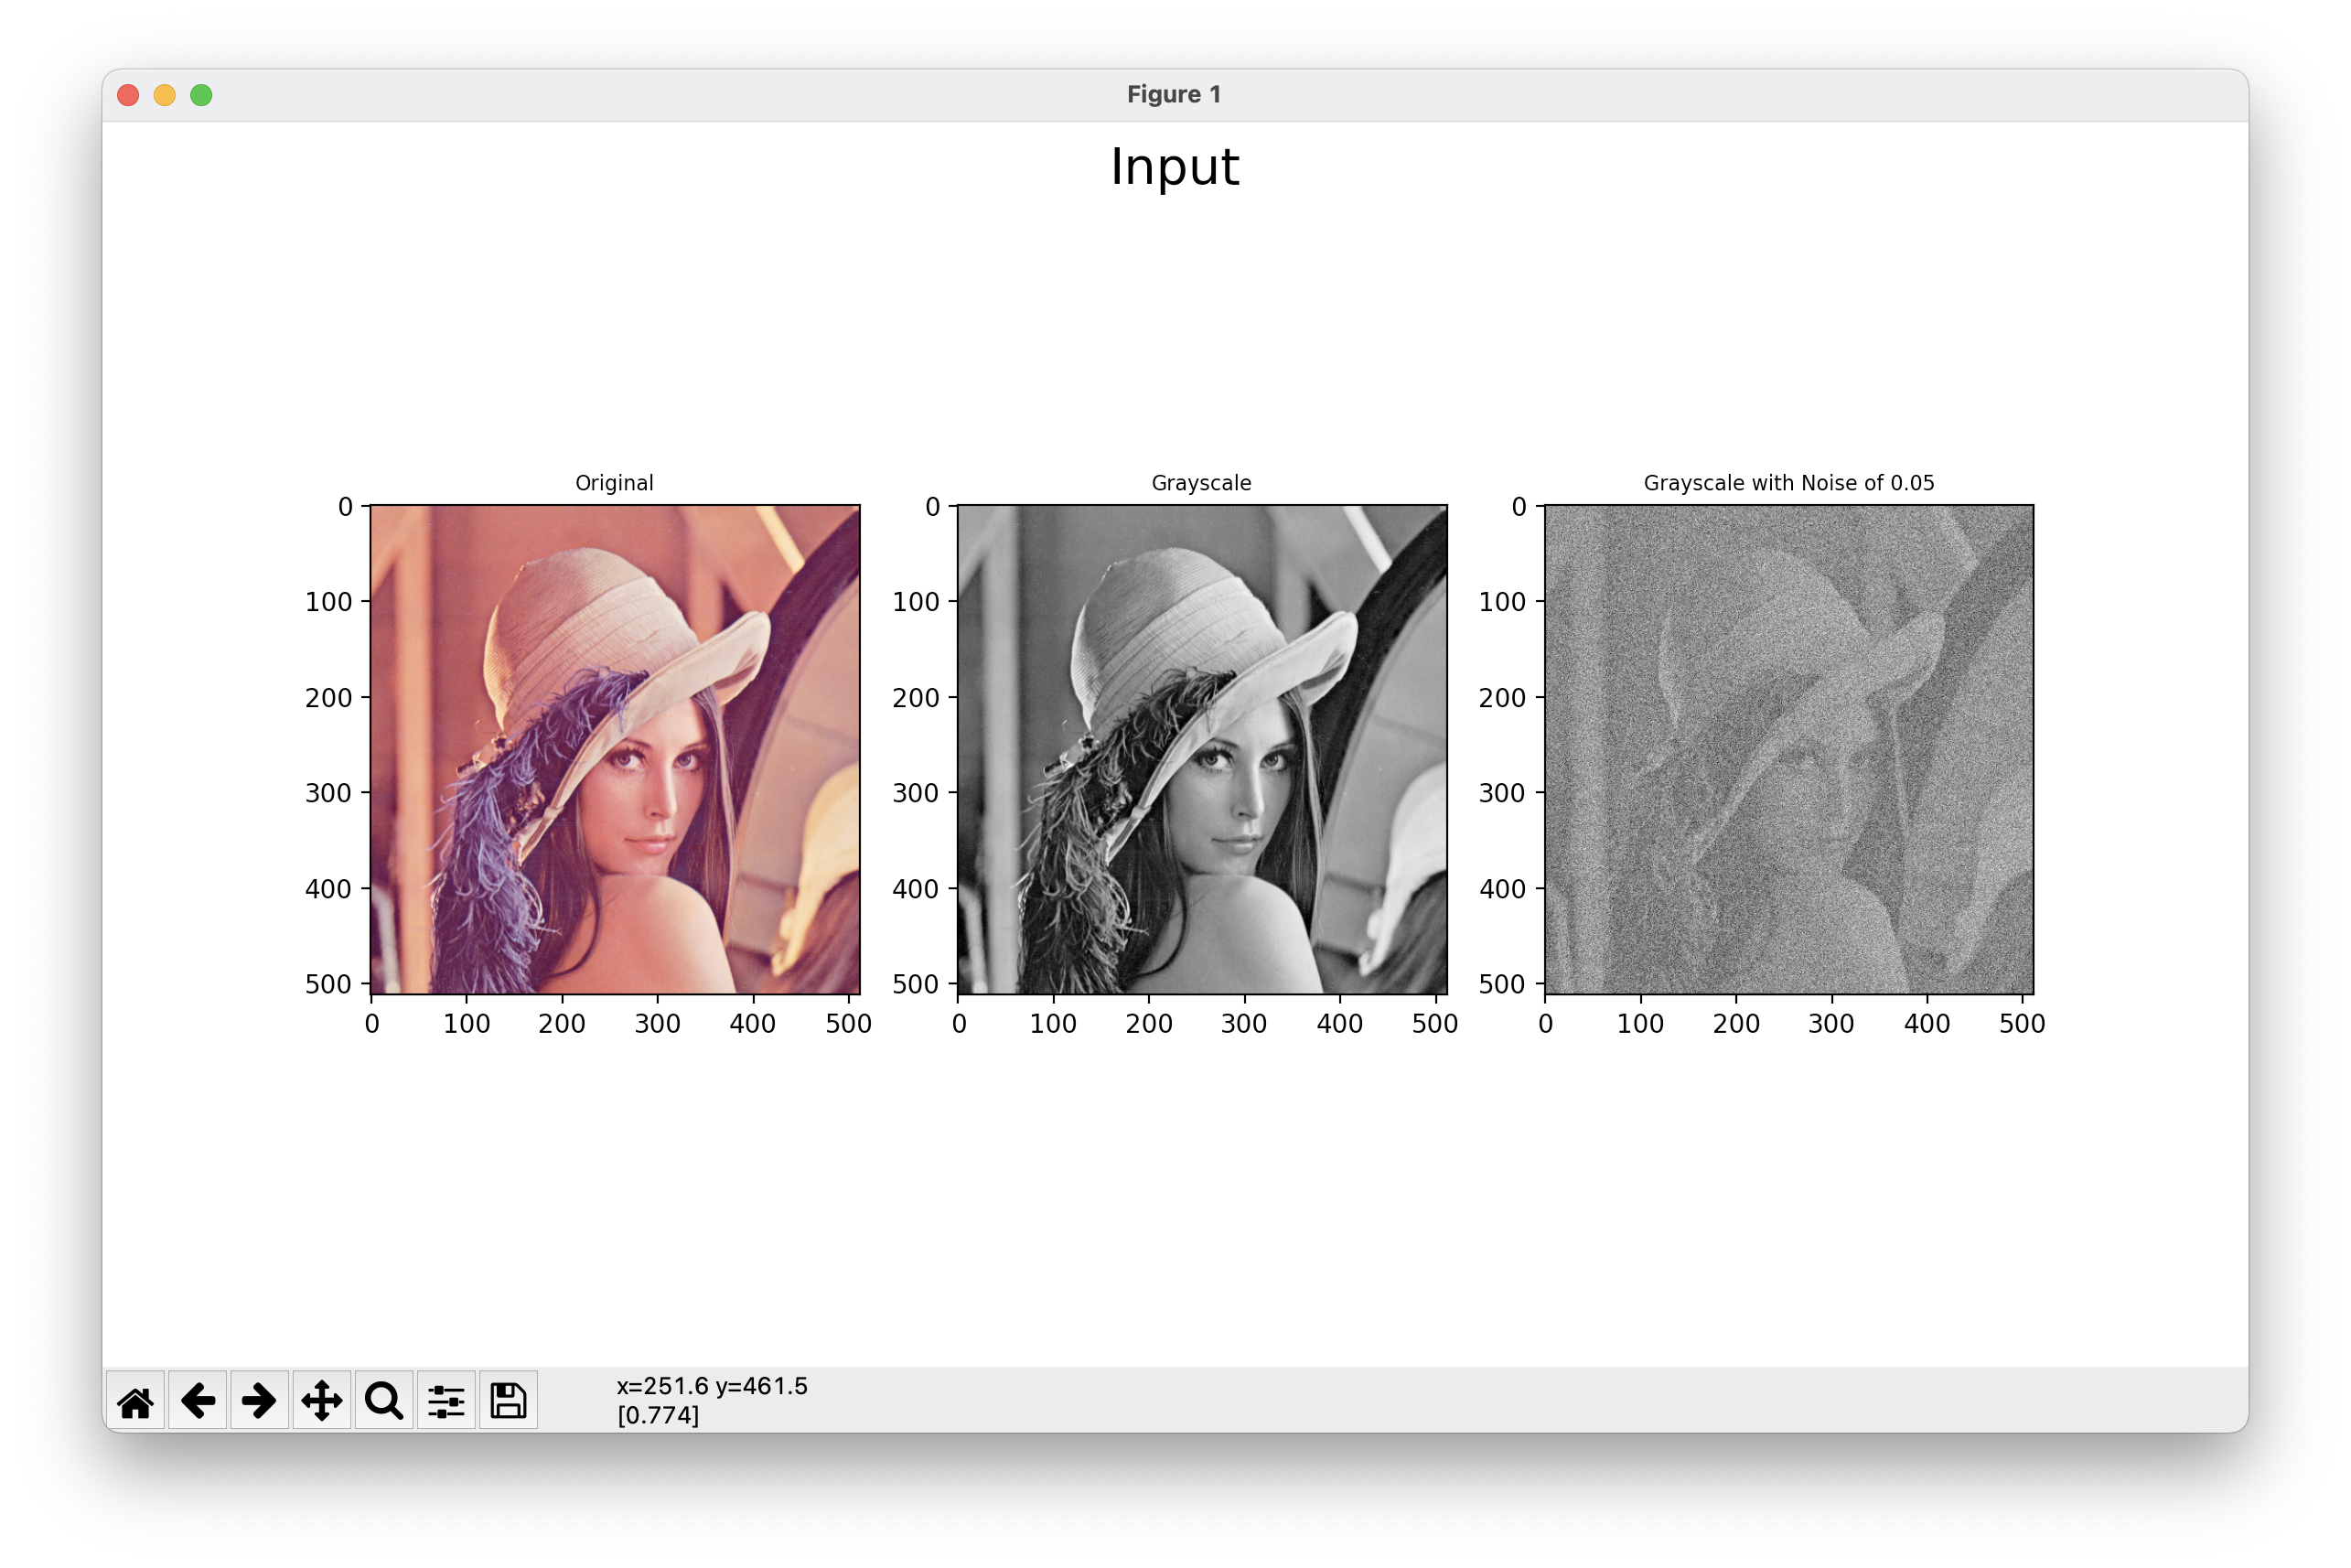
\includegraphics[scale=0.195]{3 0.05 Noise In.png}
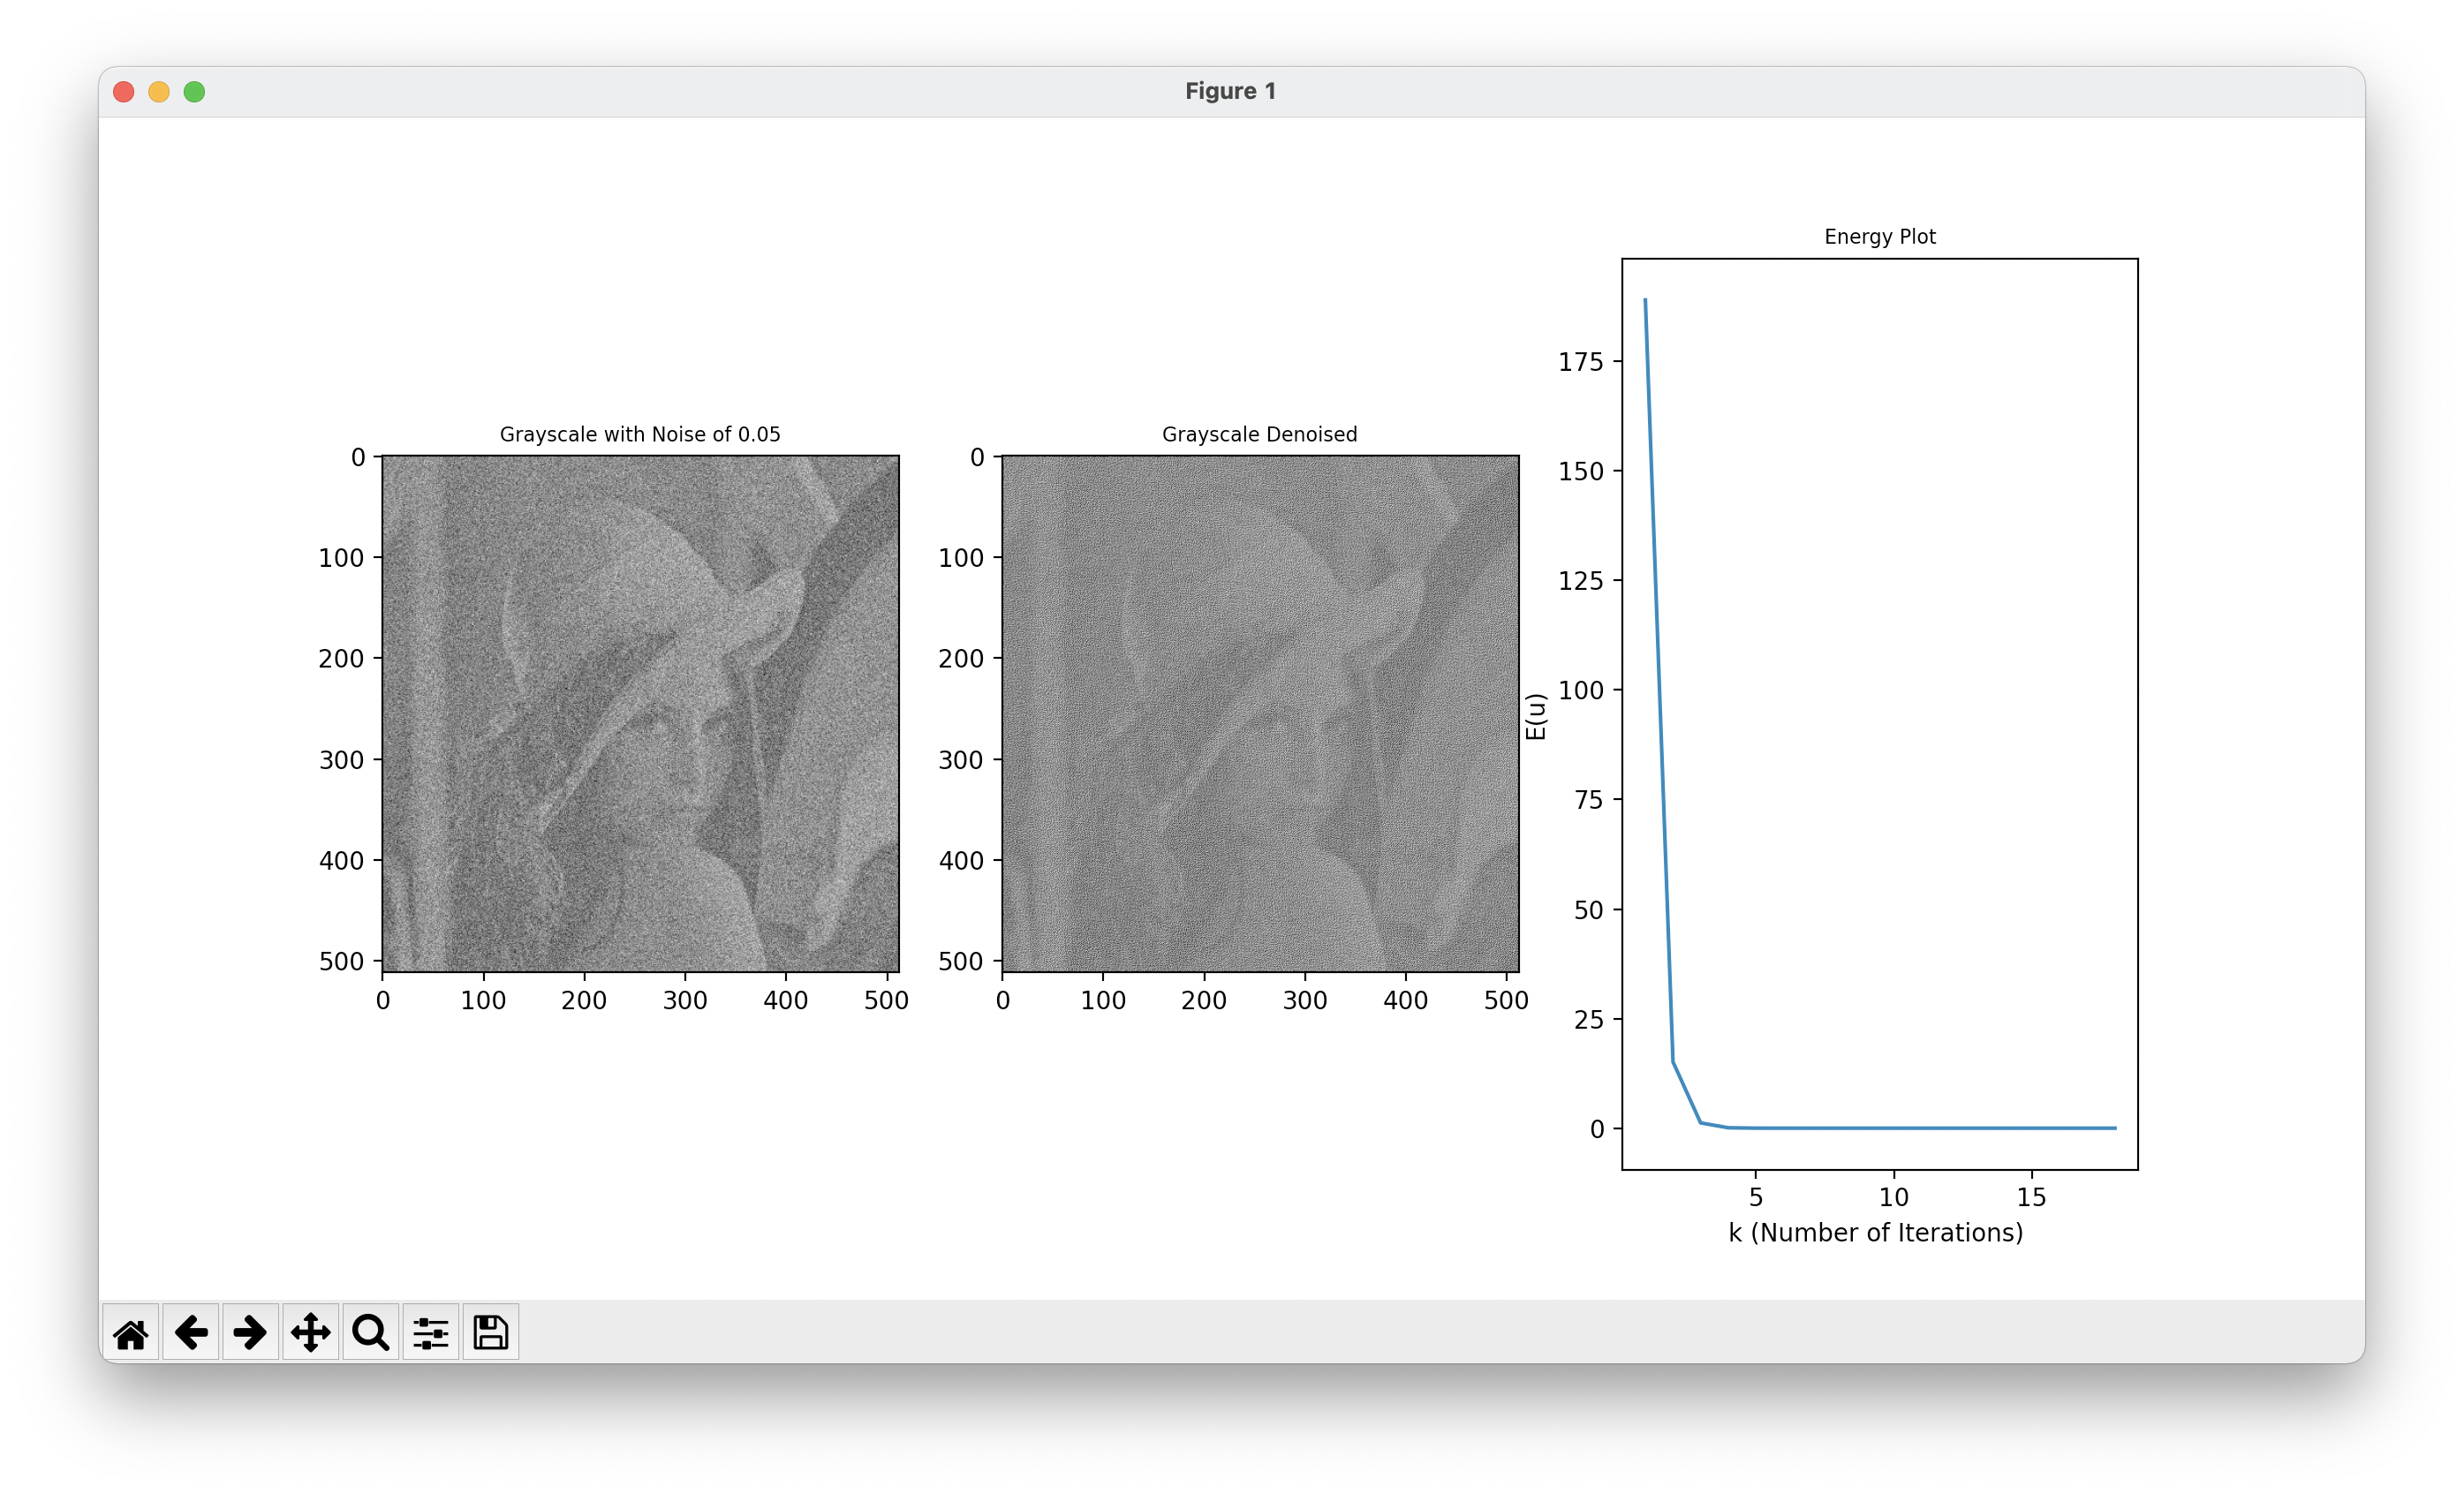
\includegraphics[scale=0.19]{3 0.05 Noise Out.png}\\\\
\noindent The following are our results from $\sigma = 0.1$\\
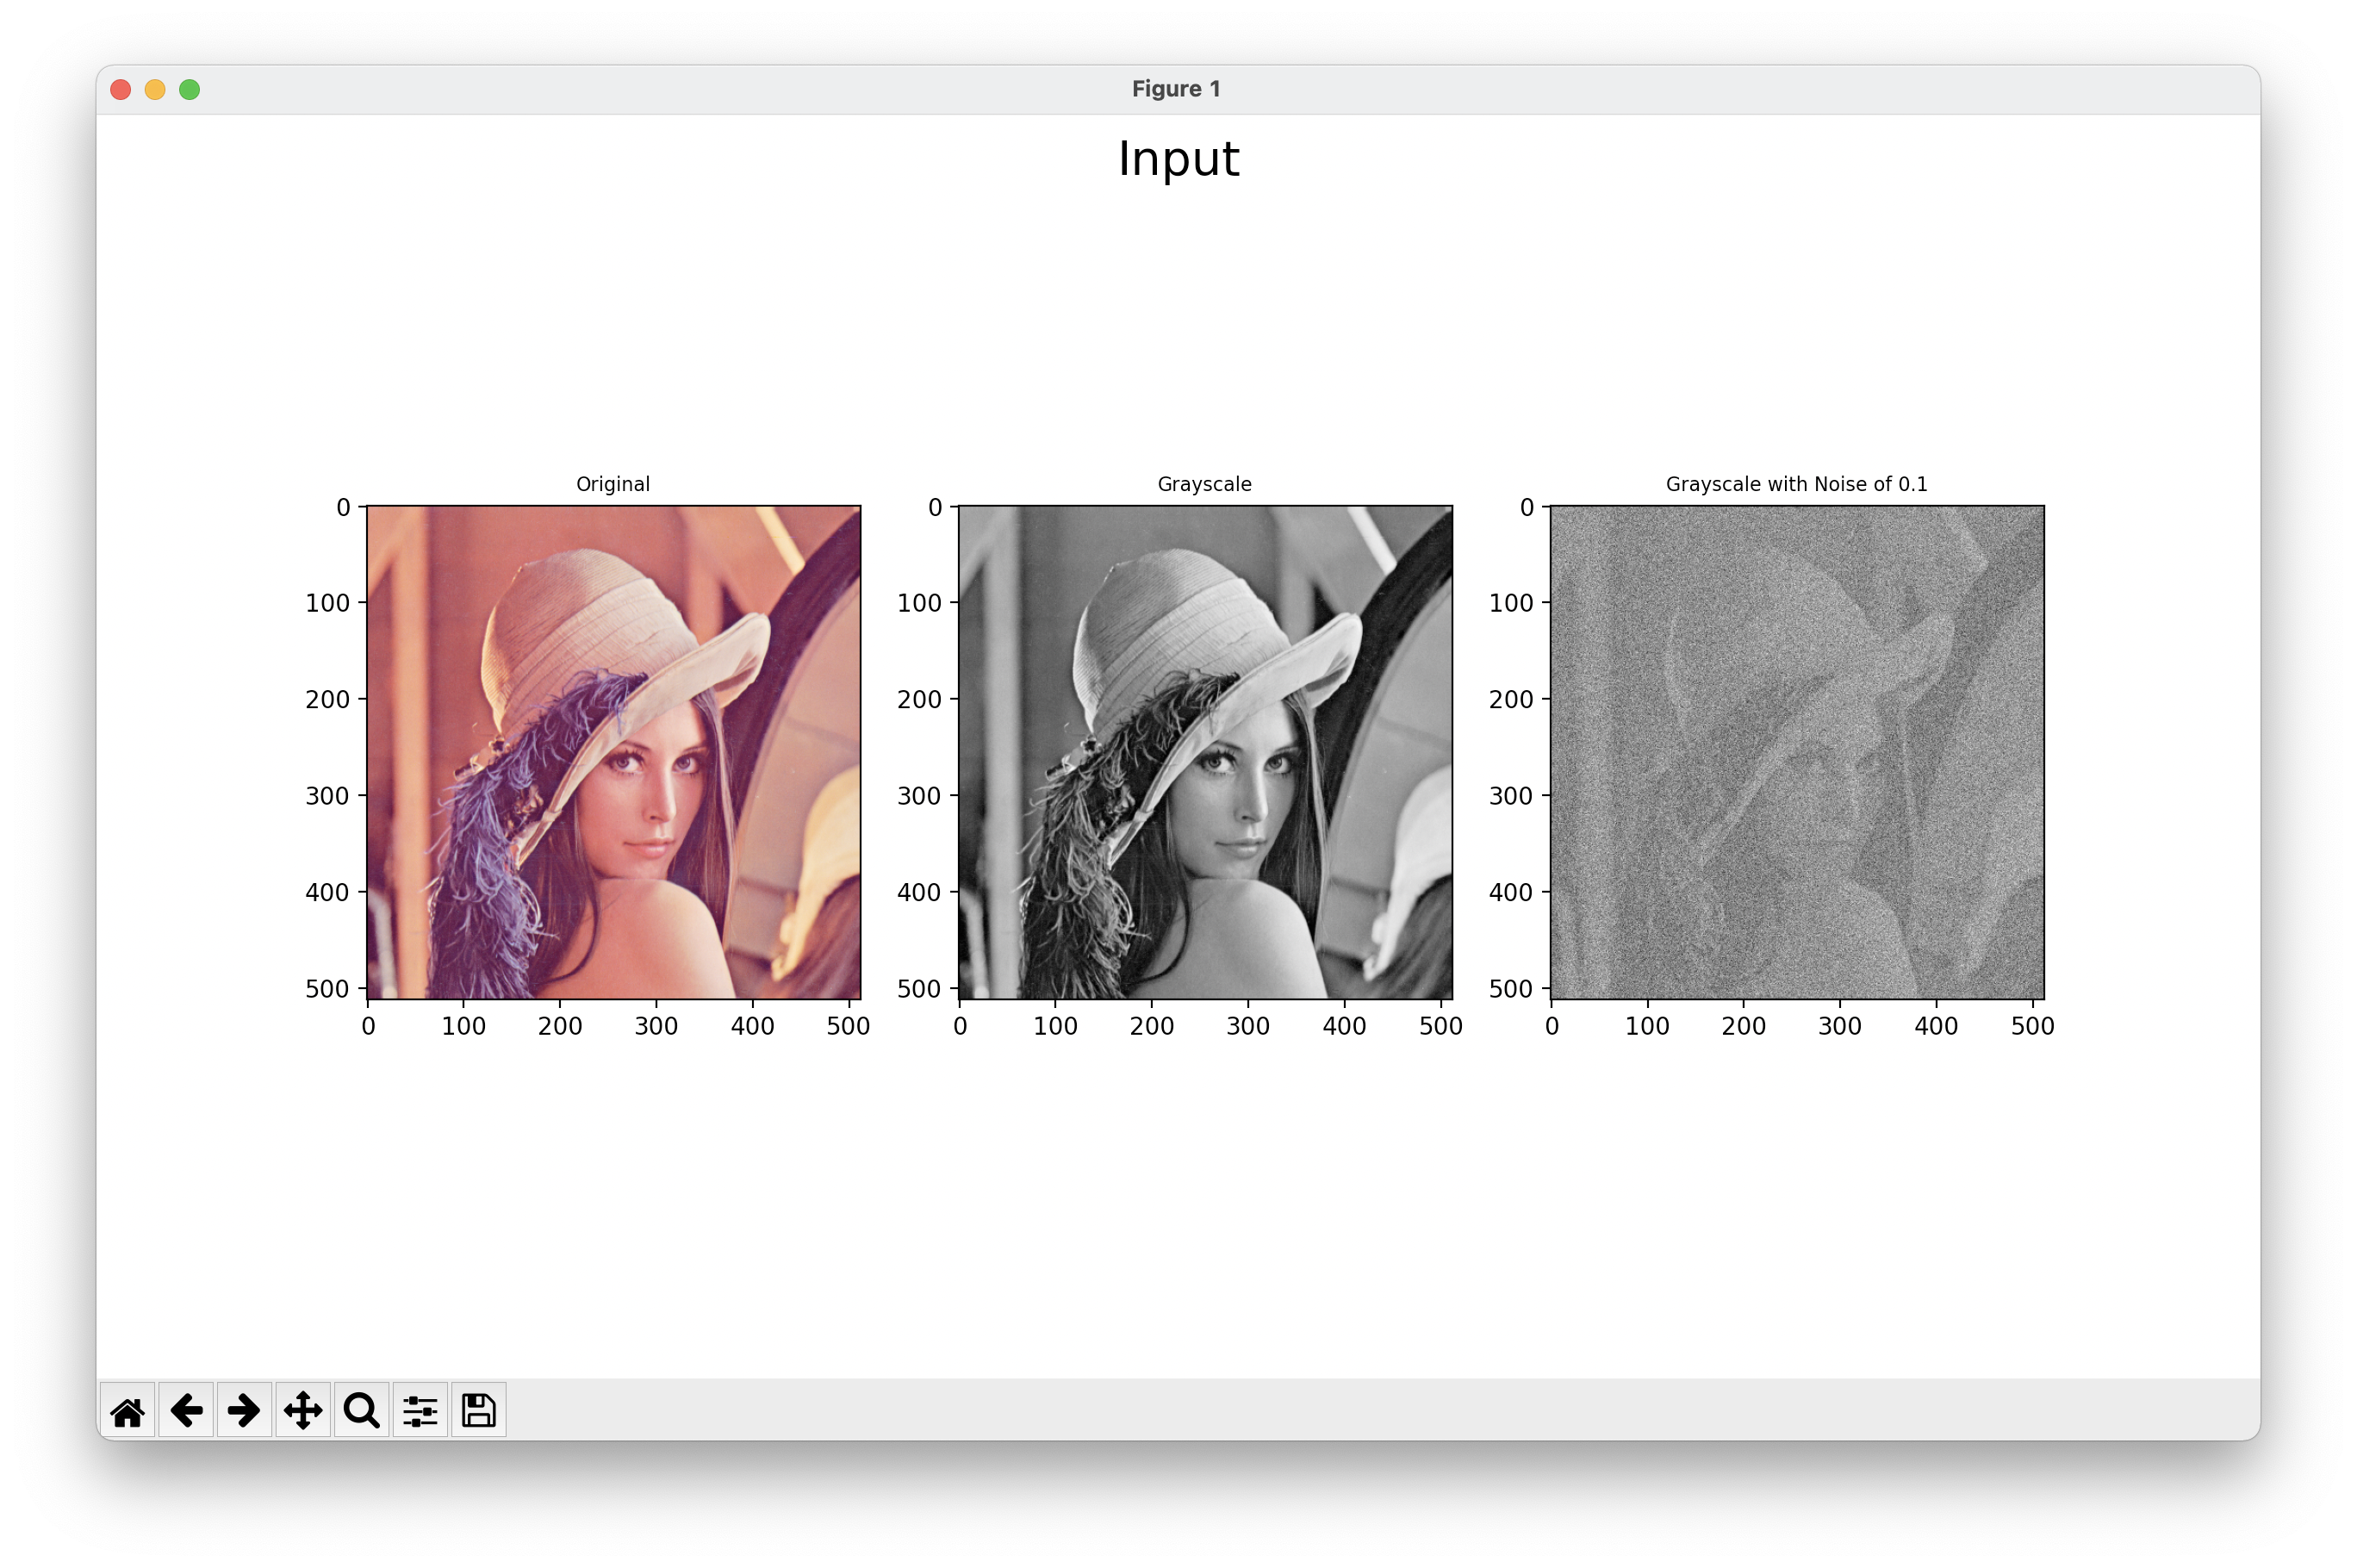
\includegraphics[scale=0.18]{3 0.1 Noise In.png}
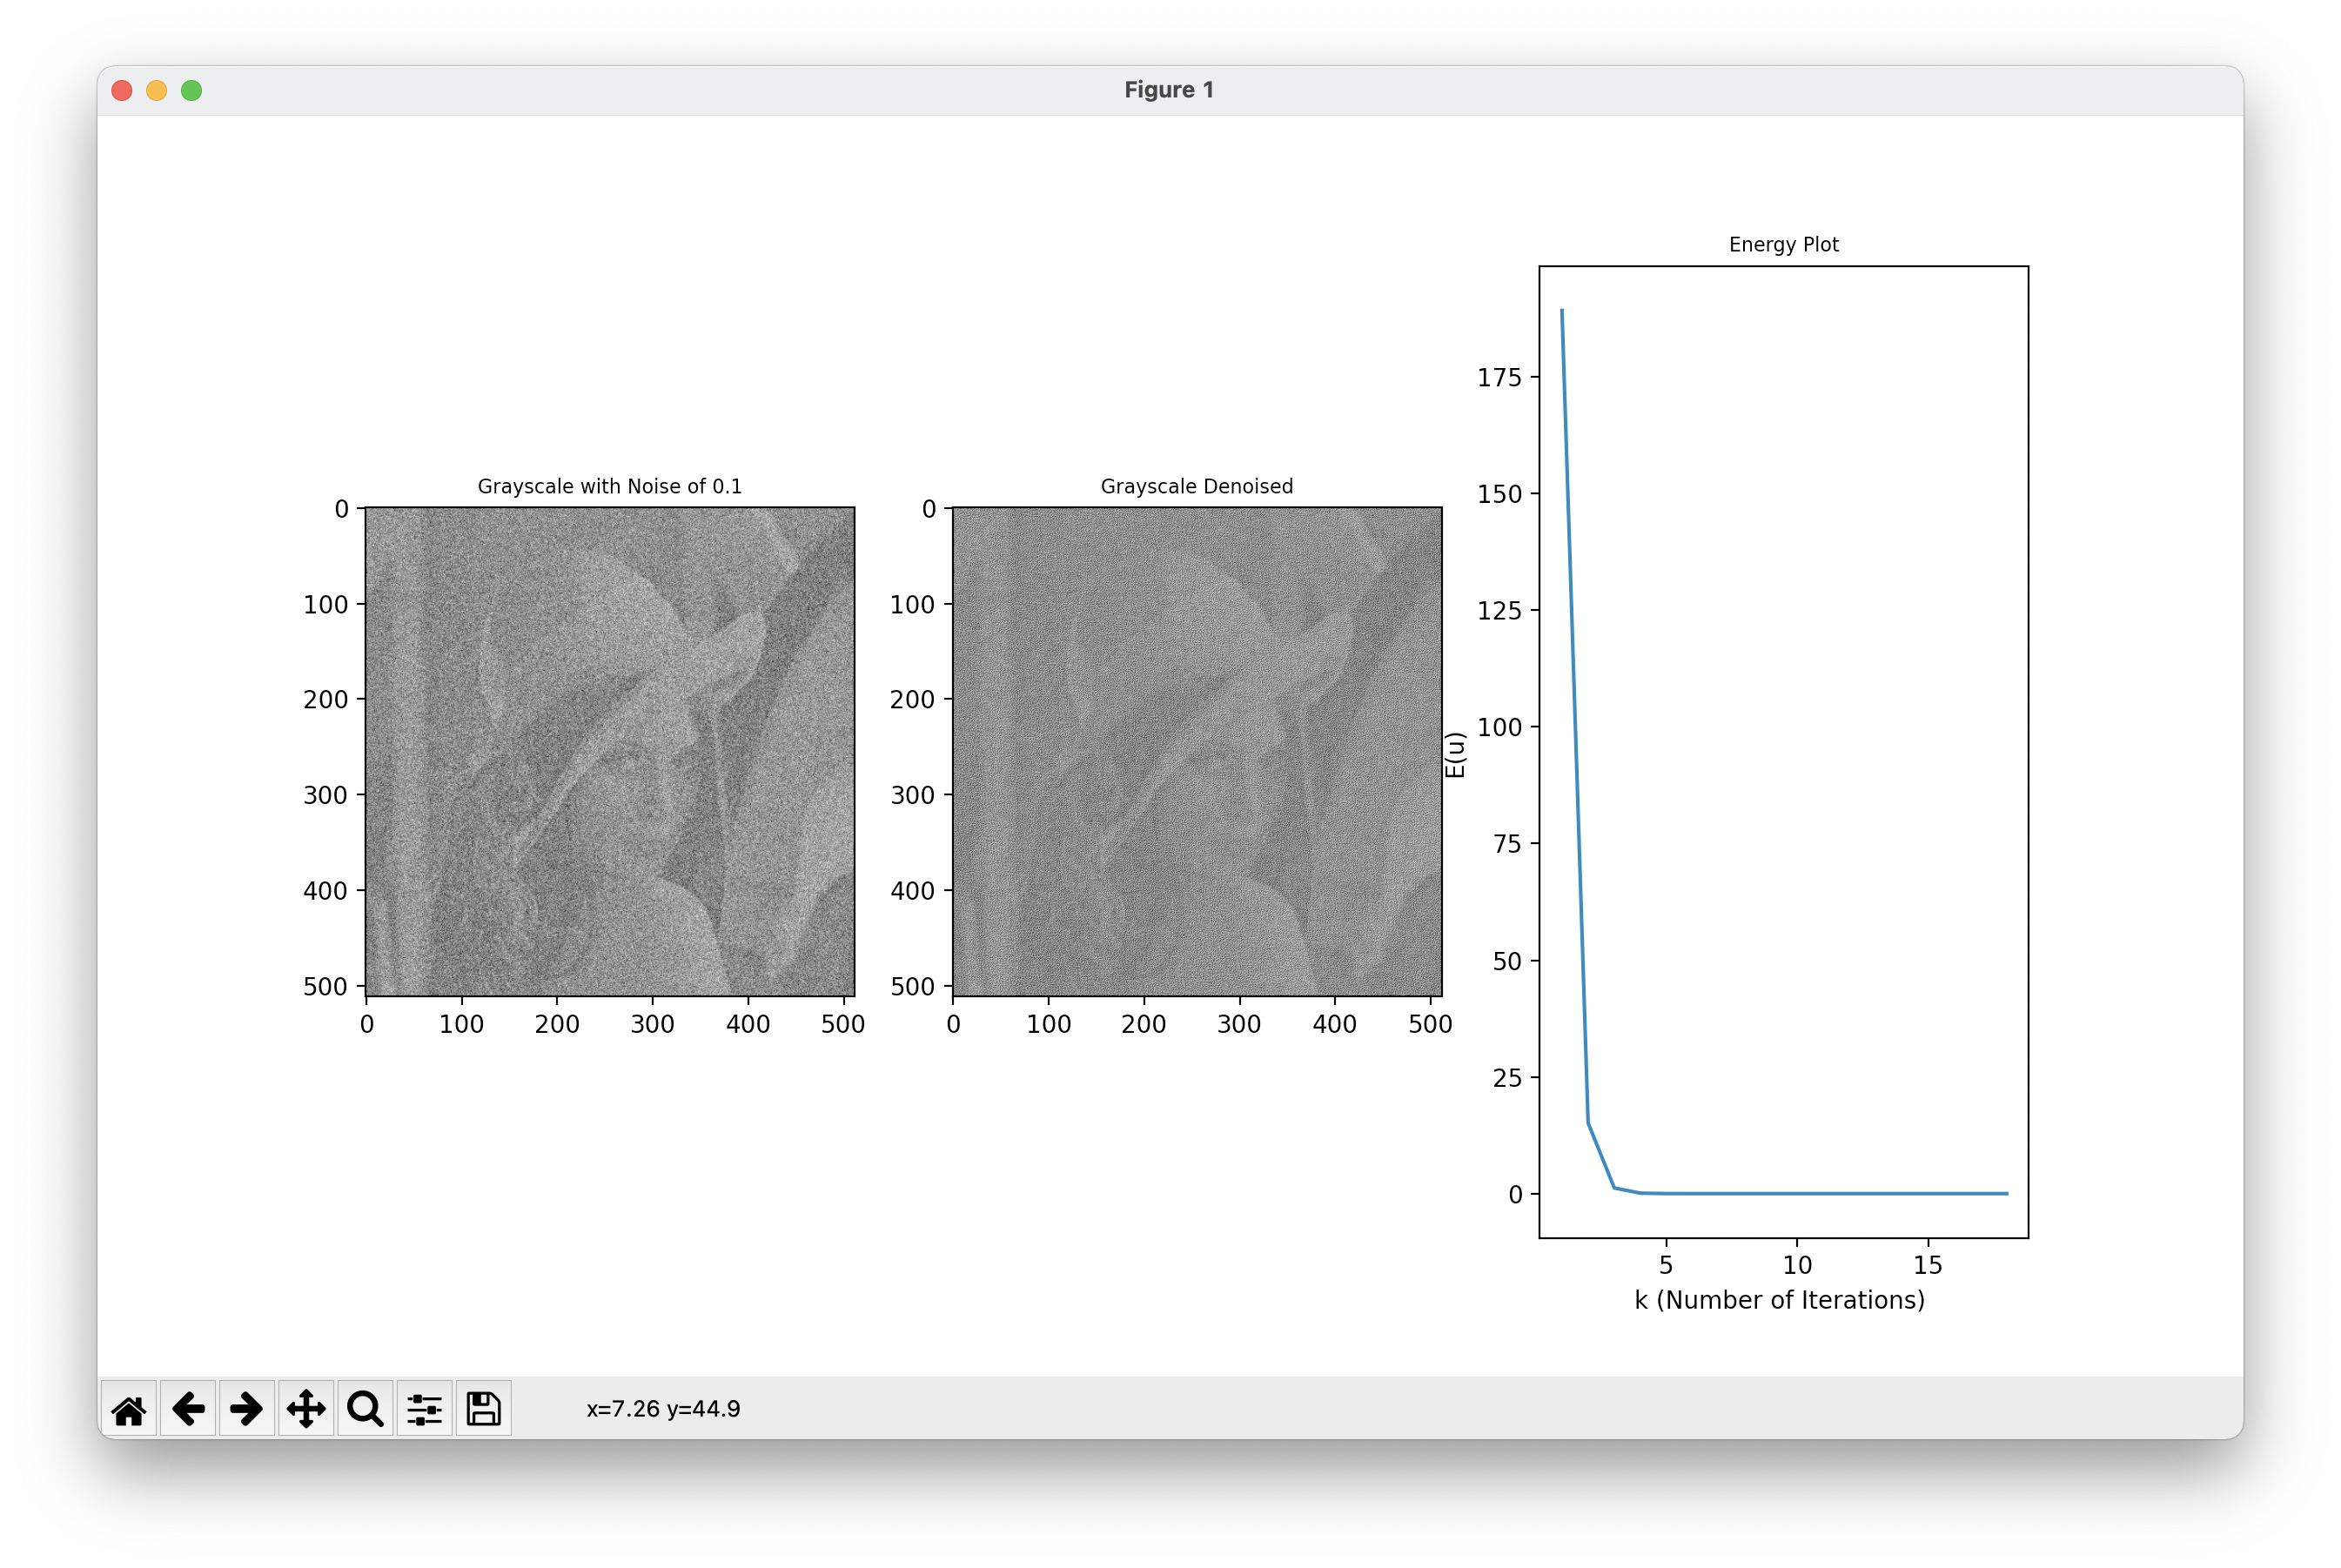
\includegraphics[scale=0.18]{3 0.1 Noise Out.png}\\\\

\noindent All graphics can be found within the root directory of the Problem Set 1 submission to be viewed at full scale.
\end{document}



\iffalse
Copy pasta below for inserting blocks of code

\begin{mdframed}[backgroundcolor=bg]
\begin{minted}{python}
\end{minted}
\end{mdframed}
\;
\;

\fi